\documentclass[12pt]{report}
\usepackage[utf8]{inputenc}
\usepackage{graphicx}
\usepackage{subcaption}
\graphicspath{ {img/} }
\usepackage{blindtext}
%\usepackage{harvard}
\usepackage{lipsum}
\usepackage{mathtools}
\usepackage{listings} % to include R-code in appendix
\usepackage{comment}
\usepackage[sectionbib]{natbib} % doesnt work
%\usepackage{float}
%\usepackage[caption=false]{subfig}
\usepackage{lmodern}
\usepackage{caption}
\usepackage{floatrow}
\usepackage{pgfplots}
%\usepackage{csquote}



\title{
	{Unit Root Tests for Panel Data}\\
	{\large University of Strathclyde \linebreak}\\
	{
\includegraphics[scale=0.25]{university.jpg}}
}
\author{Jakub Kasan}
\date{23rd August 2017}



\begin{document}
	\maketitle
		\renewcommand{\bibname}{}
	\begin{abstract}
		Stationarity testing on single time series has existed for some time in mainstream literature, but panel data stationarity tests are a relatively new field, having only been introduced around the turn of the century. It is well known that for single time series, the conventional unit root tests such as the Augmented Dickey-Fuller and Phillips-Perron lack power when the series is shorter than 100-150 observations. This means that they are unlikely to be of any use in any venue where macroeconomic data is involved, as the frequency is likely to be monthly or quarterly, meaning that decades of data would be needed to overcome the low power of the traditional tests. This is the motivation behind panel data tests, which introduce a cross dimension, and therefore can overcome the data length limitation.
		
		This paper examines the claim that panel unit root tests add power by comparing results from both single time series and panel tests done on the same data, followed by a Monte Carlo simulation on a variety of data dimensions with controlled Data-Generating Processes. The tests utilized are the Augmented Dickey-Fuller and Phillips-Perron from the single time series tests and the Levin-Lin-Chu, Im-Persaran-Shin and Maddala-Wu from the panel data tests.
		
		We find that panel data tests add power when compared to single time series tests, especially when the time dimension is short, with the provision that the cross section is large (at least 50). Compared to each other, it is clear that the Levin-Lin-Chu performs best in terms of minimizing both Type I and Type II errors.
		
	\end{abstract}

	\tableofcontents


	\chapter{Introduction}
	
The panel data format has been of great interest to the field of econometrics in general. Adding the additional dimension opens the door for analysis and inference which may not be possible with the traditional single-dimension format. The effect of adding the cross section dimension to a panel is akin to increasing the sample size, meaning that inferences made on the basis of the sample parameters are more likely to resemble the population parameters \citep{smith}. An important property which a dataset needs for inferences to be valid is stationarity, and a long-standing issue with conventional stationarity tests is that they lack power for series which are short \citep{oh1996purchasing}. A proposed solution to this issue is to pool data in the form of panels and test the entire panel \citep{llc}. For econometrics at least, this has the advantage of allowing one to work with data in the time series format (as is the convention with most econometric analysis), while having increased data and power resulting from the inclusion of a cross-section \citep{baltagi2001nonstationary}. One of the main drivers in investigations into panel data stationarity is the analysis of economic growth and the disparity between different countries. The issues regarding the panel data stationarity test are two-fold: specification of the alternative hypothesis and dealing with cross sectional dependence. The first issue deals with whether the alternative hypothesis states that the entire panel is stationary or only a majority of it is stationary. The second issue deals with the phenomenon of having a panel which has correlations across the cross section. Over the last decade or two, there have been several very thorough surveys which have detailed the current state of panel data stationarity testing in light of the two issues mentioned earlier, for example the \citet{hurlin}, \cite{baltagi2001nonstationary} or \citet{hlouskova} to name a few. These papers have split the field of panel data stationarity tests into two generations: the first during which the alternative hypothesis (or indeed null hypothesis itself, in the case of \citet{hadri2000testing}) is formulated, and then the second generation, which attempts to deal with the presence of cross sectional dependence.

This paper examines and tests a real-world dataset provided by an industrial partner using selected panel unit root tests, and then performs Monte Carlo simulations on a controlled dataset which exposes the unit root tests to a controlled process in order to determine the conditions under which each test performs best, specifically the dimensions of the panels. The reason for the Monte Carlo simulations was to put context on the results obtained from the real world data. The Monte Carlo simulations were run 10,000 times on panels ranging from 8 observations of 2 individuals to 25 observations of 50 individuals, with the $\rho$ coefficient of 0.5, 0.75, 0.9 and 1. The cross section limit was intentionally larger than the time series limit due to the fact that this is an investigation into the benefits which arise from adding the cross section dimension to panels, for cases where the time series dimension is limited, as such a limitation was the original motivation for developing panel unit root tests \citep{hurlin}. The range for the $\rho$ coefficient was chosen in order to map the sensitivity of the tests to the degree of auto-regression, as well as the ability to distinguish a stationary process from one with a unit root.

Overall, this paper found that of the three tests considered, Levin-Lin-Chu, Maddala-Wu and Im-Pesaran-Shin, the Levin-Lin-Chu performed the best in terms of minimizing both type I and type II errors. The original (flawed) implementation of the Maddala-Wu tended heavily towards type II errors while the corrected version tended heavily towards type I errors. The Im-Pesaran-Shin performed erratically with small dimensions (initially moving further from the rejection region as T grew) but then converged at acceptance levels. The Im-Pesaran-Shin test also did not show a great deal of sensitivity to whether a process had a unit root or was very close to having a unit root, overall suggesting that either the implementation was flawed or the  Of the three tests, Levin-Lin-Chu was most likely to correctly distinguish between a unit root and a stationary process, especially as the time dimension moved beyond 16 observations, which is when the Levin-Lin-Chu would converge wholly in non-rejection territory (above 10\%). Maddala-Wu performed slightly worse, as it tended to give type 2 errors with a small sample size. Regardless, all three panel data tests performed better than the single-time series tests performed on the same data.

The rest of this paper is organised as follows: the Chapter 2 goes through the literature of panel data stationarity tests and establishes the current state of the field. The Chapter 3 deals with the raw real data, its structure and characteristics as well as those of the simulated data. The Chapter 4 details the methodology of this paper, including some of the coding conventions, as this was a major part in this investigation. The Chapter 5 details the results of both the real data tests as well as the findings of the Monte Carlo simulations, followed by an informed analysis and explanation which examines the results in light of the literature discussed in chapter two. Finally, Chapter 6 evaluates the work done and offers suggestions for further investigation.



	
	\chapter{Literature Review}
	
\section{Panel Data Format}


The panel data format has been of great interest to the field of macroeconomics and beyond, largely due to the increased degrees of freedom that the format offers \citep{hsiao}. Traditionally, data was presented either as a single time series or a large cross-sections, both being one-dimensional. The issue with these one-dimensional formats is the limit of information either of them can convey. For example, if one wished to observe the impact of an event (such as the introduction of a social policy) on a number of variables (such as macroeconomic indicators), one could either measure the change in each variable individually as a separate time series, or only plot the cross section of the variables at a single point in time. This limitation is overcome by introducing an additional dimension to the data, allowing for both a time and cross-section element, which is particularly well suited to macroeconomic analysis where a wide variety of indicators are tracked over time \citep{hsiao}. As a result, the panel data format is far more powerful when compared to one-dimensional data \citep{hsiao}. The panel data format was originally developed for survey data, to collect a number of variables across several individuals \citep{smith}.  It allows for a more accurate inference of model parameters, controlling the impact of omitted variables, and generating more accurate predictions for individual outcomes by pooling the data \citep{hsiao}. As the data for this work consists of concurrent samples from the same population over time, placing it in a panel data format will allow for more power when performing statistical tests of making inferences, taking advantage of the additional samples to more accurately approximate the population parameters \citep{smith}. % Furthermore, as the individual units of the data can be considered independent, it can be assumed that the central limit theorem can be used across the cross-sectional units, demonstrating that the limiting distribution of estimators is asymptotically normal.


\section{Stationarity}


Stationarity of data is an important consideration before making any inferences and/or predictions about the underlying processes, as a non-stationary process with a unit root will be purely stochastic and will not follow a pattern \citep{dickey1986unit}. Stationarity can be split into two forms: strict stationarity or trend stationarity. Strict stationarity states that a process will oscillate over a mean of zero as $T \to \infty$ with a constant variance. Trend stationarity relaxes the zero-mean assumption, and only requires that the process oscillates over a trend. Both forms require a constant variance over $T$, however. In this work, a process will be considered "stationary" if it meets the requirements of trend stationarity. A more concrete way to describe stationarity is to consider the stochastic term in the equation, $\epsilon_t$. $\epsilon_t$ is assumed to be i.i.d. with a mean of 0 and a standard deviation of 1 ($N(0,1)$), meaning that a series described by:

\begin{equation}
	y_t = \epsilon_t
\end{equation}

should be tend towards zero as $T \to \infty$. When an autoregressive term in introduced, however, the series begins change, depending on the value of $\rho$. An autoregressive equation can be written as follows:

\begin{equation}
y_t = \rho Y_{t-1} + \epsilon_t
\end{equation}

Note that in this case, if $\rho < 1 $ and $T \to \infty$, the series will remain stationary around a zero mean (note that this is strict stationarity). The first difference of the process is described below:

\begin{equation}
	\Delta y_t = (\rho - 1) y_{t-1} + \epsilon_t
\end{equation}

In the case of $\rho < 1$, the differenced process retains a deterministic component ($y_{t-1}$), and is stationary around a constant mean. If $\rho = 1$, then the deterministic component turns to zero and the only component left is the stochastic component, and the process becomes non-stationary, as the integrated process ($y_t$) will effectively become $y_t = \sum_{i=1}^{T}\epsilon_t$, where the variance is non-constant, thus violating the stationarity assumption. All stationary tests therefore attempt to correctly specify the $\rho$ value in the autoregressive process, in order to determine if the process is indeed stationary around zero (or a level or trend) or has a unit root, in which case it can also be described as being integrated to the order one, or I(0).

\subsection{Augmented Dickey-Fuller}

The first major unit root test introduced was the Dickey-Fuller (DF) test, which tested a null hypothesis of a unit root in the series versus an alternative hypothesis of no unit root \citep{df}. This test assumed that the series followed the form expressed in figure 2.3.

Another assumption of this test is that the series is zero-mean and that the lag order is known. Both assumptions are limiting for real-world application, and therefore an augmented version (ADF) was proposed \citep{said1984testing}. This version offered an additional two models: one with a drift (2.4) and the other with a drift and trend (2.5).

\begin{equation}
y_t = \alpha + \rho y_{t-1} + \epsilon_t
\end{equation}

\begin{equation}
y_t = \alpha + \beta t + \rho y_{t-1} + \epsilon_t
\end{equation}

The procedure for the Augmented Dickey-Fuller is as follows. First, a regression is estimated where the lag order is set so that the $\epsilon_t$ terms are uncorrelated. The selection of the lag order is perhaps the most important part of the test, as if the lags are too few, the errors will have serial correlation while if the lags are too many, the test will lose power \citep{hlouskova}. One such way of selecting the appropriate lag order was detailed by \citet{ng1995unit} and their method is as follows: a value for the maximum permissible lag order is chosen arbitrarily, and then regressions are performed sequentially from that value to a lag order of zero. If the absolute value of the t-statistic of the last lagged difference ($\Delta y_{t-i}$) is greater than 1.6, the procedure is halted, the current lag order is considered correct, and the unit root test is performed. An approach for selecting the maximum permissible lag order was suggested by \citet{schwert}, where the value is set as:

\begin{equation}
P_{max} = 12 * (\cfrac{T}{100})^{\cfrac{1}{4}}.
\end{equation}


\subsection{Phillips-Perron}

Another unit root test was proposed by \citet{pp}. This test was remarkably similar to the Augmented Dickey Fuller test, except for in the way that it dealt with serial correlation. While the ADF uses a parametric autoregression to find the structure of errors, the Phillips-Perron test corrects the initial test statistic to account for the possible presence of serial correlation. As a result, the Phillips-Perron test is non-parametric, not requiring the specification of a lag structure, but is asymptotic, meaning that under finite samples will perform worse than the Augmented Dickey-Fuller, \citep{davidson2004econometric}. The null hypothesis for the Phillips-Perron, as with the Augmented Dickey-Fuller, is the presence of a unit root, versus an alternative of a stationary time series \citep{pp}.

\subsection{Kwiatkowski-Phillips-Schmidt-Shin}

Compared to the Phillips-Perron and the (Augmented) Dickey-Fuller, the Kwiatkowski-Phillips-Schmidt-Shin test has a null hypothesis of stationarity, with the alternative being unit root \citep{kpss}. Also unlike the Dickey-Fuller or Phillips-Perron tests, the data-generating process form is slightly different, being expressed as:

\begin{equation}
y_t = \xi_t + \epsilon_t
\end{equation}

The $\xi_t$ is a random walk while $\epsilon_t$ is stationary. In addition:

\begin{equation}
y_t = \xi_t + \epsilon_t
\end{equation}

Where $v$ is i.i.d with a mean of 0 and standard deviation equal to $\sigma^2$. If the variance is zero, in other words if $\sigma^2 = 0$, then $\theta_t = \theta_0$ for all $t$ and the process $y_t$ is stationary.

\section{Panel Data Stationarity}

Examining stationarity in panel data as opposed to time series data presents a number of challenges, the chief of which is the specification of the tests. With a single time series test, the series is either considered stationary or not stationary, which is not a problem. With panel data, however, the possibilities are slightly more complex: a panel can have all members be stationary, some be stationary, or none be stationary. This presents a problem for the practical use of a test.\\ If we consider two panel data unit root tests, they may both have a null hypothesis of all the series having a unit root, but they may have different alternative hypothesis: one may state that all the series are stationary (referred to as the homogeneous case), the other that at least one of the series is stationary (the heterogeneous case). In practice, it is generally accepted that macro-economic panel data usually consist of a mix of stationary and non-stationary time series \citep{hurlin}, which is why a major consideration with panel data is the specification of the alternative hypothesis: are all members of the panel stationary or just majority? \\Another challenge with panel data unit root tests is the issue of heterogeneous or homogeneous $\rho$ coefficients. Some tests are flexible and allow heterogeneity in the coefficients while others (such as the Levin-Lin-Chu) do not. The preference for either model must be governed by assumptions about the data. If the data consists of samples from the same population (as it is in the case of this work) it may be wise to force the same $\rho$ coefficient on all the individuals. However, in the case of distinct variables (such as with macro-economic panels), allowing heterogeneity in the $\rho$ coefficients may produce a better model. \\Another issue which affects panel data unit root tests is the presence (or lack thereof) of cross-sectional correlation in the data. A critical assumption of many of the early proposed panel data tests was that the individuals were not correlated, but in a practical setting this was severely limiting as many applications where the panel data format was used it was used specifically because the individual components had some degree of correlation \citep{panic04}. Over time, new tests robust to cross-sectional dependence were developed, and the literature splits the panel data unit root tests into two “generations,” the first which assumes cross-sectional independence and the second which does not.

\subsection{First Generation Tests}
The first generation tests can be divided into two rough categories: the first which combines statistics of individual tests (such as \citet{mw} or  \citet{ips}) or those which create a combined statistic from the entire panel (such as the \citet{llc}). The main point of focus with the first generation, however, is whether the alternative hypothesis is homogeneous or heterogeneous, which is to say if the alternative states that the entire panel is stationary, or if only some of the panel is stationary.

\subsubsection{Maddala and Wu 1999}

Maddala-Wu 1999 proposed a test which was based on the methodology first proposed by \citet{fisher}. This method involves combining the p-values of the individual unit root tests done on each individual in the panel. This test is robust to heterogeneous lag orders, $\rho$ values, even choice of test, as only the p-value was necessary. Crucially, this test is implementable on unbalanced panels. The test statistic is given by:

\begin{equation}
P_{MW} = -2 \sum_{i=1}^{N} \log p_i
\end{equation}

The test statistic follows a $\chi$-squared distribution with $2N$ degrees of freedom, as $T \to \infty$. The simplicity of this test and its robustness to a wide variety of factors (as stated above) make it very attractive \citep{banerjee1999panel}.

\subsubsection{Harris and Tzavalis 1999}

The Harris and Tzavalis test is unique among the first generation of panel unit root tests because while most are designed so that $T \to \infty$ quicker or at the same rate that $N \to \infty$, the HT test considers the case where $T$ is fixed and $N \to \infty$ \citep{harris1999inference}. The null hypothesis is that the DGP has a unit root, and the distribution under the null hypothesis is unaffected by the nuisance parameters (trend and intercept). Harris and Tzavalis show that the limiting distributions of the test statistics are normal and that their convergence rate is the same as for the case of stationary panel data ($\sqrt{N}$).

\subsubsection{Hadri 2000}

The test proposed by Hadri is an adaptation of the KPSS test for the panel format \citep{hadri2000testing}. Unlike all the other first generation tests, the null hypothesis here is that the panel is stationary, with an alternative of a unit root. The test has two models; either the process is stationary around a deterministic level or the process is stationary around a deterministic trend.





In these models, $r_{i,0}$ is the heterogeneous intercept, $\beta$ is the time trend coefficient while $\epsilon_{i,t}$ is $\sum_{j=1}^{T} u_{i,j}+ \epsilon_{i,j}$. $r_{i,t}$  is a random walk and is “i.i.d.” with a mean of zero and a standard deviation of $\sigma_u^2$. Under the null hypothesis, $\sigma_u^2 = 0$ and $\epsilon_{i,t}$ is stationary. If $\sigma_u^2 \neq 0$, then $\epsilon_{i,t}$ is non-stationary and the $r_{i,t}$ term from the equations above is a random walk.  The test statistic for Hadri is:

\begin{equation}
Z_\mu = \cfrac{\sqrt{N}-E[\int_{0}^{1}V(r)^2dr]}{\sqrt{V[\int_{0}^{1}V(r)^2dr]}} ,
\end{equation}

where

\begin{equation}
LM = \cfrac{1}{\sigma_{\epsilon}^2} * \cfrac{1}{NT^2}(\sum_{i=1}^{N} . \sum_{t=1}^{T} S^2_{i,t})
\end{equation}

\subsubsection{Choi 2001}

This test is an expansion of the original Maddala-Wu 1999 test \citep{choi2001unit}. \citet{choi2001unit} proposes a standardized statistic for panels where the N dimension is large, which is given below:

\begin{equation}
Z_{MW} = \cfrac{\sqrt{N}\{N^{-1}P_{MW}-E[-2\log(p_i)]\}}{\sqrt{Var[-2log(p_i)]}} = \cfrac{\sum_{i=1}^{N}+N}{\sqrt{N}}
\end{equation}

Under the unit root hypothesis and assuming that the cross-section is independent, this statistic converges to a standard normal distribution.

\subsubsection{Levin et al 2002}
\citet{llc} proposed different panel data test, building on the model they developed (as Levin and Lin) in 1997, which tested the null hypothesis of a unit root against a heterogeneous alternative of stationarity in all the data individuals \citep{llc}. The models which are considered by \citet{llc} are the zero-mean, intercept and trend with intercept.

The procedure begins with an Augmented Dickey-Fuller test on all the individuals to select the lag order and coefficients $\cite{df}$. Then, two sets of residuals are saved, one from regressing ($\Delta y_{i,t-1}$ on $\sum_{j=1}^{L} \Delta y_{i,t-j} + \alpha + \beta t$ where $L$ is the number of lags specified) that becomes $\bar{e}$, the other from regressing $y_{i,t-1}$ on $\sum_{j=1}^{L} \Delta y_{i,t-j} + \alpha + \beta t$) that becomes $\bar{f}$. The residuals are standardized using the standard error, $\sigma$ which is calculated from regressing $e_t$ on $f_t$ , creating the standardized residuals, $\hat{e}$ and $\hat{f}$. Next, the ratio of long-run variance to the short-run variance of $\Delta y_{i,t}$ is estimated. Long-run variance is defined as:

\begin{equation}
\sigma^2_{ui,LR} = \sigma^2_{ui} + 2 * \sum_{j=1}^{\infty}E(u_{it}u_{i,t-j})
\end{equation}

which leads to the estimated expression:

\begin{equation}
\hat{\sigma}^2_{ui,LR} = \cfrac{1}{T}\sum_{t=1}^{T}\hat{u}^2_{it} + \cfrac{2}{T} \sum_{j=1}^{L}\omega (j, L) \sum_{t=j+1}^{T} \hat{u}_{it}\hat{u}_{i,t-j}
\end{equation}

The individual ratio of long-run to short-run variance is therefore defined by:

\begin{equation}
\hat{s}^2_i = \hat{\sigma}^2_{ui,LR} / \hat{\sigma}^2_{ui}
\end{equation}

With:

\begin{equation}
\hat{\sigma}^2_{ui} = \cfrac{1}{T} \sum_{t=1}^{T} \hat{u}^2_{it}
\end{equation}

The test statistic is computed by the following formula:

\begin{equation}
\hat{\Phi} = \cfrac{\sum_{i=1}^{N}\sum_{t=p_i+2}^{T}\hat{e}_{it}\hat{f}_{it-1}}{\sum_{i=1}^{N}\sum_{t=p_i+2}^{T}\hat{f}^2_{it-1}}
\end{equation}



Ultimately, there are three separate cases for which a test statistic can be compared to a t-statistic distribution, the zero-mean, intercept and trend models. For the zero-mean model, it has been shown that the t-statistic is asymptotically N(0,1) (Hlouskova and Wagner, 2005). For the intercept and trend case, the t-statistic diverges and has to be normalized and re-centered so that it converges to a limiting distribution using the formula below:

\begin{equation}
t_{\phi}^*=\cfrac{t_{\phi}-N\tilde{T}\hat{S}_{NT}STD(\hat{\phi})\mu_{mT}}{\sigma_{mT}}
\end{equation}



\subsubsection{Im, Pesaran and Shin 2002}

Im, Pesaran and Shin proposed a panel data test which considered the case of either intercept-only or intercept and trend DGP and allowed for individual-specific autoregressive structures.

The test proposed by Im, Pesaran and Shin (hereafter known as IPS) is based on the Augmented Dickey-Fuller statistic similarly to the LLC. Unlike the LLC, however, IPS allow for heterogeneity with the $\rho$ coefficient in the alternative hypothesis $\cite{hurlin}$, therefore some of the individuals can have a unit root in the alternative hypothesis. The IPS model assumes either a model with a time trend and/or intercept. This test is somewhat similar to the Fisher-type tests proposed by Maddala and Wu (1999) and Choi (2001), where the data is not pooled, but rather the Augmented Dickey-Fuller statistic is averaged across the panel, which is expressed as:

\begin{equation}
\bar{t}_{NT} = \cfrac{1}{N}\sum_{i=1}^{N}t_{iT}(p_i,\beta_i) 
\end{equation}

The authors have shown that the distribution of the test statistic converges to a normal distribution as $T \to  \infty$ and then as $N \to \infty$ $\cite{hurlin}$. Specifically, as $T \to \infty$, the individual statistic converges to the Dickey-Fuller distribution, while as $N \to \infty$ then the $\bar{t}$ statistic tends to a normal distribution. The following equation is used to standardize the $\bar{t}$ statistic, denoted as $W_{\bar{t}}$ :

\begin{equation}
	W_{\bar{t}} = \cfrac{\sqrt{N}(\bar{t}_{NT}-N^{-1} \sum_{i=1}^{N}E[t_{iT}(p_i,0)|\epsilon = 0])}{\sqrt{N^{-1} \sum_{i=1}^{N}Var[t_{iT}(p_i,0)|\epsilon = 0]}}
\end{equation}

\subsection{Second Generation Tests}

The second generation of panel unit root tests attempt to address the issue of cross-sectional dependence. Cross sectional dependence has been an often-cited issue with the first generation tests $\cite{hurlin}$, and it's presence is said to cause significant issues when dealing not just with stationarity tests, but it has even been found that the pooled Ordinary Least Squares estimator for a panel with cross sectional dependence offers little improvement over a single-equation OLS that ignores the dependence $\cite{phillips2003dynamic}$.

\subsubsection{Bai and Ng 2001 \& 2004}
Bai and Ng are credited with proposing the first test of unit root in panel data which took into account cross-sectional correlation $\cite{hurlin}$. The approach splits the process of each individual of the panel into three components: the first is the individual deterministic component which is heterogeneous, and the second “common component,” which is comprised of two vectors, one with the common factors $F_t$ and another with the factor weightings $\gamma$, and the third is the error term, $e_{i,t}$ $\cite{panic04}$. The deterministic component and the error term are unique for each individual in the panel, while the “common component” is shared across the panel and accounts for the cross-sectional process. The process is expressed as such:

\begin{equation}
y_{i,t} = D_i + \gamma_i'F_i + \epsilon_{i,t}
\end{equation}

A process, $y_{i,t}$ can be considered non-stationary if either one of the factors in the vector $F_t$ is non-stationary or if the error term is non-stationary. Due to the fact that if the process contains a large stationary component then checking the stationarity of the process as a whole becomes difficult, the procedure suggested by Bai and Ng tests the common and individual components separately. They call this procedure PANIC (Panel Analysis of Nonstationarity in the Idiosyncratic and Common components) $\cite{panic04}$. The major downside to this procedure is the fact that the common factors $F_t$ and error terms $\epsilon_{i,t}$ need to be estimated, and the power of the PANIC procedure depends on the estimators. Assuming that these estimators can be correctly estimated, however, this test can address the complaints regarding cross-sectional dependency typically expressed about the "traditional" panel unit root tests such as the Levin-Lin-Chu $\cite{hurlin}$.

%\subsubsection{Phillips and Sul 2003}

%The test proposed by Phillips and Sul


\subsubsection{Moon and Perron 2004}

A similar procedure to the one described by $\cite{panic04}$ was detailed by $\cite{moon2004testing}$. This procedure, similarly to $\cite{phillips2003dynamic}$, does not test the individual or common factors for the presence of a unit root. $\cite{moon2004testing}$ consider the following model:

\begin{equation}
y_{i,t} = \alpha_i + y_{i,t}^0 ,\\
\end{equation}
\begin{equation}
y_{i,t}^0 = \phi  y_{i,t-1}^0 + \mu_{i,t} ,\\
\end{equation}
\begin{equation}
\mu_{i,t} = \lambda' F_t + \epsilon_{i,t} .\\
\end{equation}

The $\phi$ component is tested for the presence of a unit root, and the hypotheses are as follows: \\
\linebreak
$H_0 : \phi = 1, \forall i = 1, ..., N$ \\
$H_1 : \phi < 1$ for at least one individual $i$. \\
\linebreak

The approach that $\cite{moon2004testing}$ take here is to eliminate the effect of the common components on the series $y_{i,t}$ entirely before applying the unit root test. Thereby the cross-sectional dependencies are removed, which means that normal asymptotic distributions are obtained, similarly to $\cite{llc}$ or $\cite{ips}$. The exception being that the test statistics here are independent in the individual dimension. The authors propose two seperate test statistics which converge together as $T$ and $N$ tend to $\infty$ and $N/T$ tends to $0$. The test statistics are:

\begin{equation}
%t_a = T \sqrt{N} (\hat{\phi}_{\alpha}^{\plus} - 1)
t_a = \cfrac{T \sqrt{N} (\hat{pool}_{\alpha}^{+} -1)}{t_b = {\sqrt{2 \gamma_{\epsilon}^4/\omega_{\epsilon}^4}}} \lim_{{T,N} \to \infty}^d N(0,1) ,
\end{equation}

\begin{equation}
t_b = T \sqrt{N} ( \hat{\phi}_{pool}^{+} - 1) \sqrt{ \cfrac{1}{NT^2} trace(Z_{-1} QZ'_{-1} ) \cfrac{\omega^2_\epsilon}{\gamma_\epsilon^4}} \lim_{{T,N} \to \infty}^d N(0,1) .
\end{equation}

\subsubsection{Choi 2002}

$\cite{choi2002combination}$ fundementally differs from the $\cite{moon2004testing}$ or $\cite{panic04}$ in that there is only one common factor to account for the cross sectional dependence. Additionally, Choi assumes that each time series shares a common time trend. The basic model is:

\begin{equation}
y_{i,t} = \alpha_i + \theta_t + v_{i,t},
\end{equation}

where

\begin{equation}
v_{i,t} = \sum_{j=1}^{p_i} d_{i,j} v_{i,t-j} + \epsilon_{i,t}.
\end{equation}

The approach described by $\cite{choi2002combination}$ essentially transforms the initial panel, then calculates three statistics, which are said to be all normally distributed as $ N \to \infty$ under the null hypothesis of a unit root. The three statistics are as follows:

\begin{equation}
P_m = - \cfrac{1}{\sqrt{N}} \sum_{i=1}^{N} [ \ln {p_i} + 1 ]
\end{equation}

\begin{equation}
Z = - \cfrac{1}{\sqrt{N}} \sum_{i=1}^{N} [ \theta^{-1} (p_i)
\end{equation}

\begin{equation}
L* = \cfrac{1}{\sqrt{\pi^2 N / 3}} \sum_{i=1}^{N} \ln ( \cfrac{p_i}{1 - p_i})
\end{equation}




	
	\chapter{Data}
	\section{Real Data}

\subsection{Data Structure}

The data given by the industrial partner has been anonymised due to confidentiality agreements, and thus neither the type of the variables nor nature of the data can be disclosed. The information which can be disclosed, however, is that the raw data consisted of 979 observations of 9 variables, with the ninth variable being the one of interest. The form of the raw data was such that it was a series of panels stacked in a single column, and the frequency of the observations was quarterly (i.e. four times a year). Due to the way the statistical packages were programmed, a minimum of 8 observations had to be imposed on the data, so series which had less than 8 observations were removed. The cleaned data was therefore 36 time series: one with a length of 40, four of length 39, and then one each from lengths 38 to 8.

\subsection{Data Characteristics}

As stated, the structure of the cleaned data was a number of panels consisting of of time series, with observations ranging from 40 to 8. Before summary statistics were calculated, all the series were correctly graphed by the corresponding quarter, as seen in Graph 1.

To determine which model the data followed (zero-mean, mean or trend), a dummy variable range from one to the length of the series was regressed upon each series and the p-values for both the trend and intercept were analyzed. Of the 36 series remaining after the cleaning phase, 29 were found to have a trend at a 95\% confidence and 30 at a 90\% confidence. As stated previously, the data is assumed to have the same Data-Generating Process, ergo the remaining series which did not have high enough confidence values for the intercept term are assumed to have a trend in the DGP.

%\begin{figure}
	
%\includegraphics[scale=0.5]{paneldata.jpg}

%\end{figure}


\begin{figure}[htp]
	\centering
	\begin{subfigure}{0.75\textwidth}
		\centering
		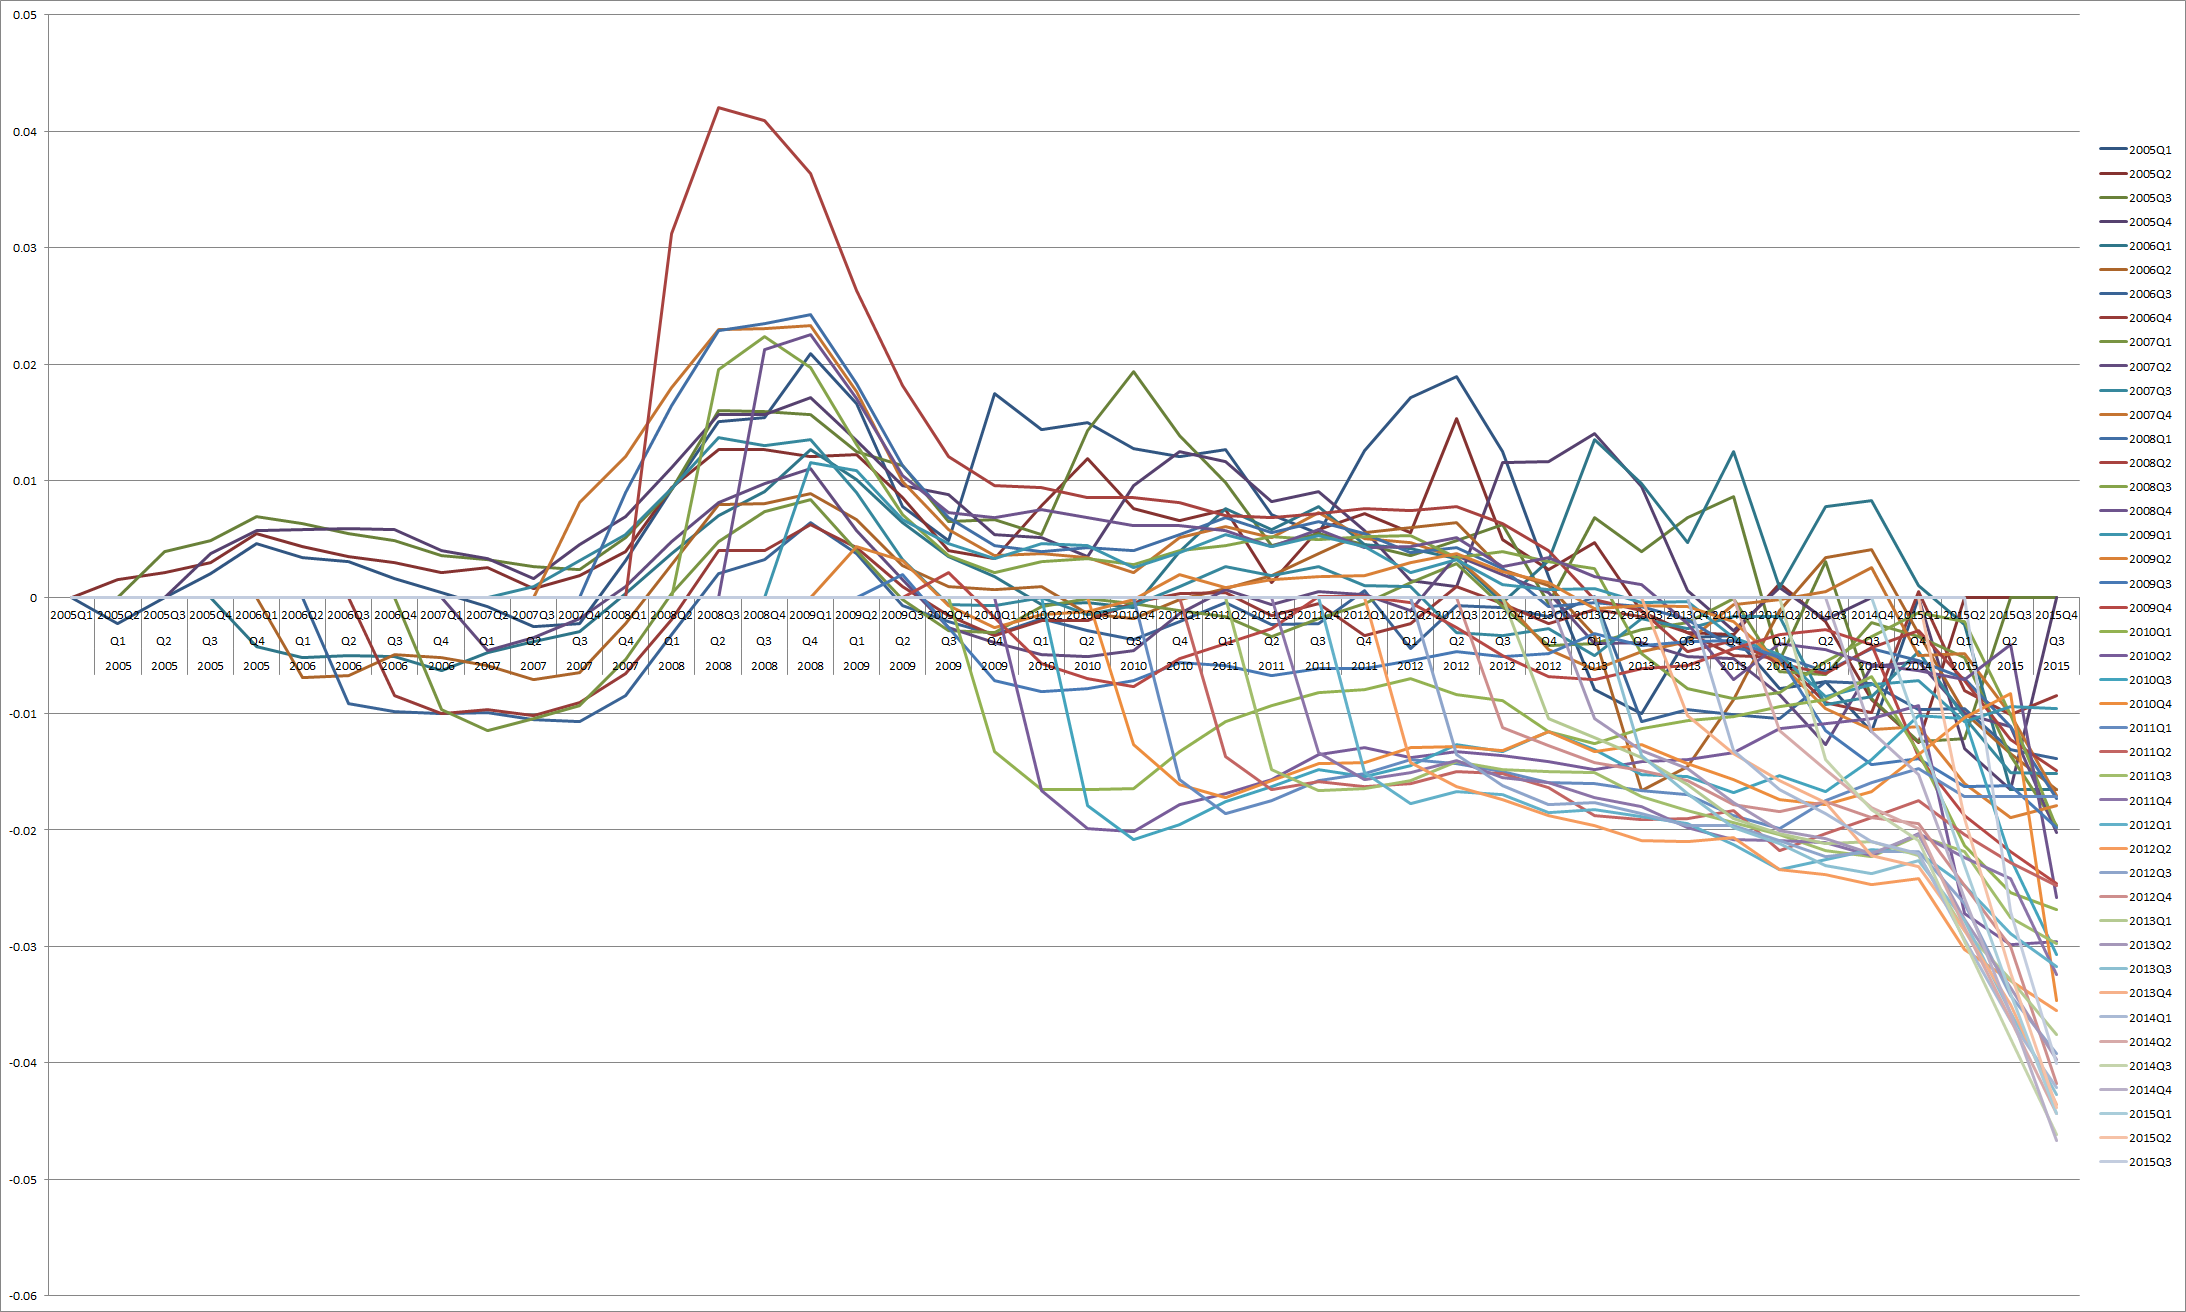
\includegraphics[width= \linewidth]{panel_graph}
	\end{subfigure}
\caption{Time series plot of all real data.}
\end{figure}

After the model was identified as having a linear trend, the next step was to identify whether or not it followed an $AR$ process. All the series were passed through the auto-correlation function and partial-auto-correlation function. On balance, the individuals all followed an autoregressive process of order one, as is visible with some of the selected ACF/PACF graphs shown below. 


\begin{figure}[htp]
	\centering
	\begin{subfigure}{0.23\textwidth}
		\centering
		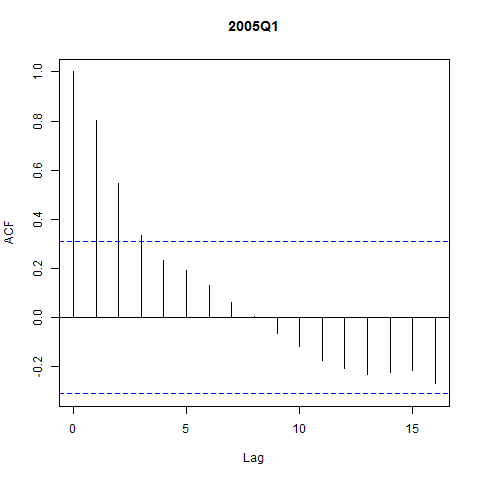
\includegraphics[width= \linewidth]{2005Q1-acf}
	\end{subfigure}
	\begin{subfigure}{0.23\textwidth}
		\centering
		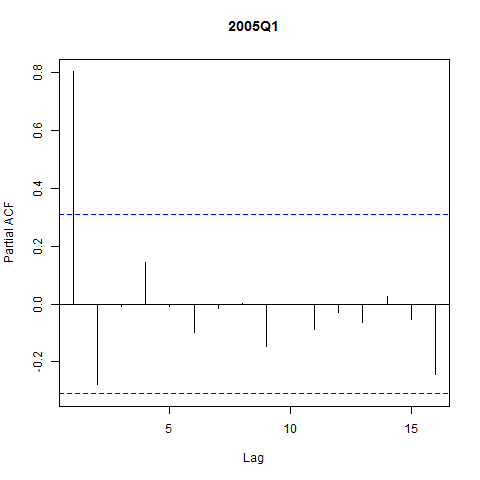
\includegraphics[width=\linewidth]{2005Q1-pacf}
	\end{subfigure}
	\begin{subfigure}{0.23\textwidth}
		\centering
		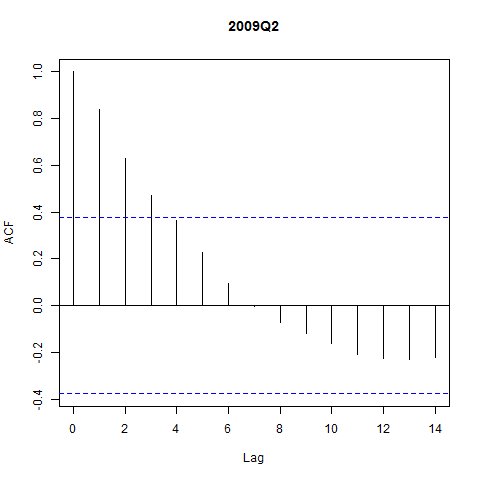
\includegraphics[width= \linewidth]{2009Q2-acf}
	\end{subfigure}
	\begin{subfigure}{0.23\textwidth}
		\centering
		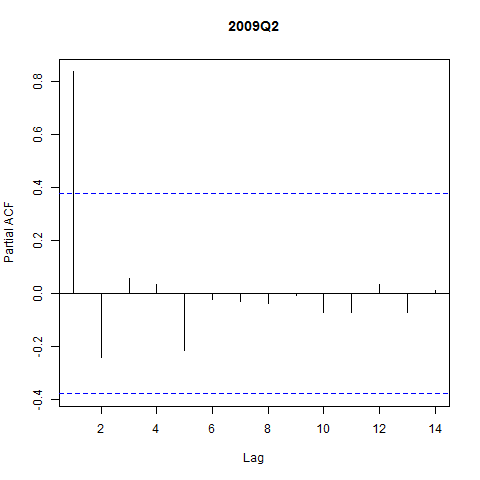
\includegraphics[width=\linewidth]{2009Q2-pacf}
	\end{subfigure}
\caption{Select ACF and PACF plots from the real data.}
\end{figure}

Again, it should be noted that the data did not uniformly show an $AR(1)$ process on the ACF/PACF graphs, but because the individuals of the panel are assumed to be samples of an identical process, it is further assumed that the few series which are not appearing as $AR(1)$ process are appearing as such due to sampling error, which is further justified by the fact that these non-conforming series are the shortest lengths, i.e. smallest sample size.


\section{Simulated Data}

\subsection{Data Structure}

The panels created for the Monte Carlo simulations ranged from a panel with 8 observations of 2 individuals to 25 observations of 50 individuals. Each individual was a bespoke AR(1) process with a $\rho$ value as specified in that instance.


\subsection{Data Characteristics}

The data used in the Monte Carlo simulations was an AR(1) process, which was simulated using R. The process can be expressed as below:

\begin{equation}
y_t = \rho y_{t-1} + \epsilon_t
\end{equation}

A range of $\rho$ values was simulated, from 0.5 to 1, in order to gauge the power of the tests. All but the last value ($\rho = 1$) are stationary time series, with the exception being non-stationary with a unit-root. With low values of $\rho$, the series is clearly deterministic around a mean (which in this case is zero) with a small degree of noise. Four sample processes are displayed below where the value of $\rho$ has been set for 0.5 and T is 10,20,100,500.

\begin{figure}[htp]
	\centering
	\begin{subfigure}{0.23\textwidth}
		\centering
		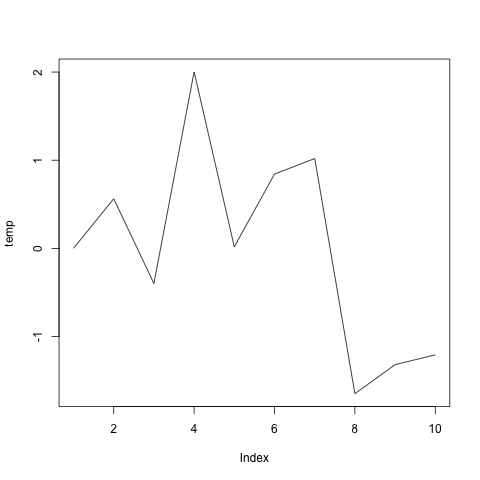
\includegraphics[width= \linewidth]{10-05-plot}
	\end{subfigure}
	\begin{subfigure}{0.23\textwidth}
		\centering
		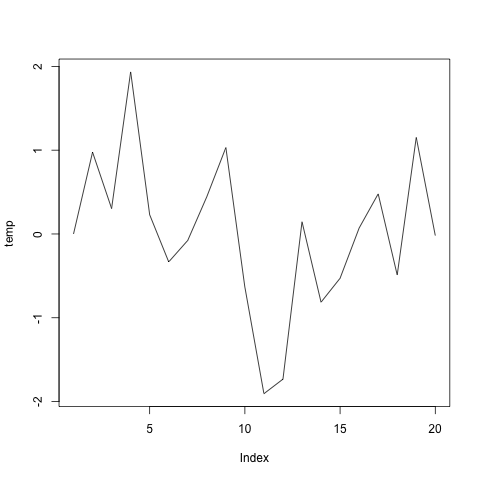
\includegraphics[width=\linewidth]{20-05-plot}
	\end{subfigure}
	\begin{subfigure}{0.23\textwidth}
		\centering
		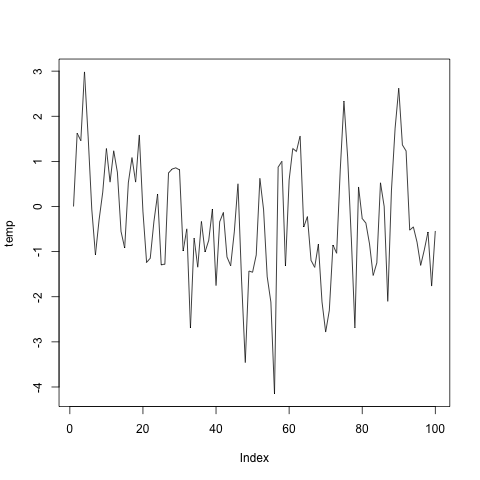
\includegraphics[width= \linewidth]{100-05-plot}
	\end{subfigure}
	\begin{subfigure}{0.23\textwidth}
		\centering
		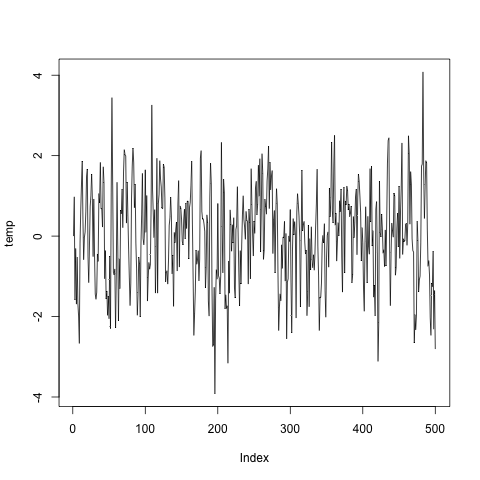
\includegraphics[width=\linewidth]{500-05-plot}
	\end{subfigure}
\caption{Time series plots for $\rho = 0.5$}
\end{figure}



Even for the processes with $T = 10$ and $T = 20$, the zero-mean trend is clearly visible, albeit with a large degree of noise. When $T = 100$ or $500$, however, the process very clearly appears stationary around a zero mean. When the ACF and PACF are applied to the data, they detect no auto-correlation for cases with $T = 10$ and $T = 20$, while for the case of $T = 100$, it is borderline and for $T = 500$ it is clear cut, as is shown in the charts below.

\begin{figure}[htp]
	\centering
	\begin{subfigure}{0.23\textwidth}
		\centering
		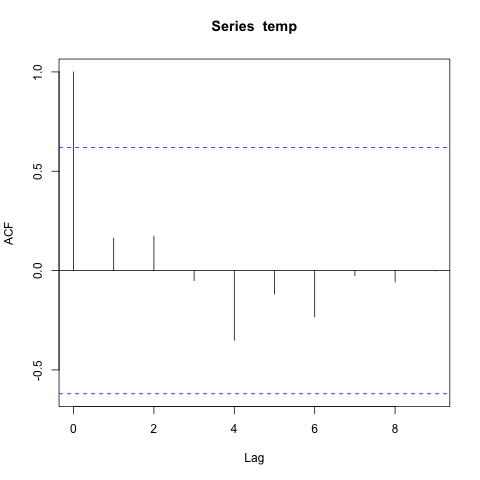
\includegraphics[width= \linewidth]{10-05-acf}
	\end{subfigure}
	\begin{subfigure}{0.23\textwidth}
		\centering
		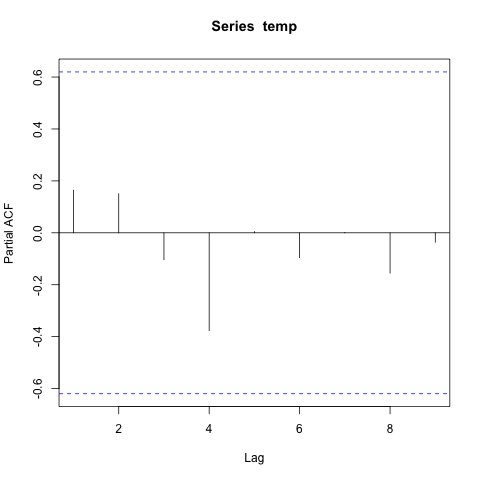
\includegraphics[width=\linewidth]{10-05-pacf}
	\end{subfigure}
	\begin{subfigure}{0.23\textwidth}
		\centering
		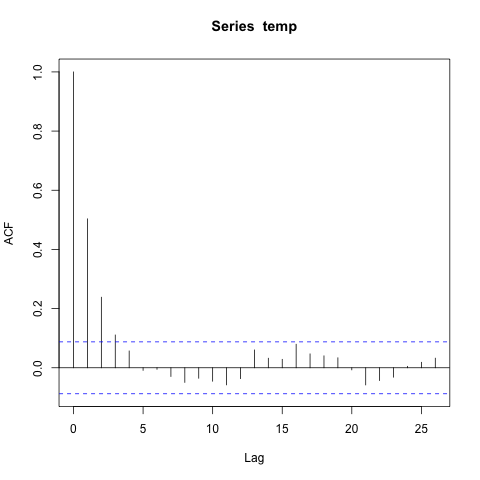
\includegraphics[width= \linewidth]{500-05-acf}
	\end{subfigure}
	\begin{subfigure}{0.23\textwidth}
		\centering
		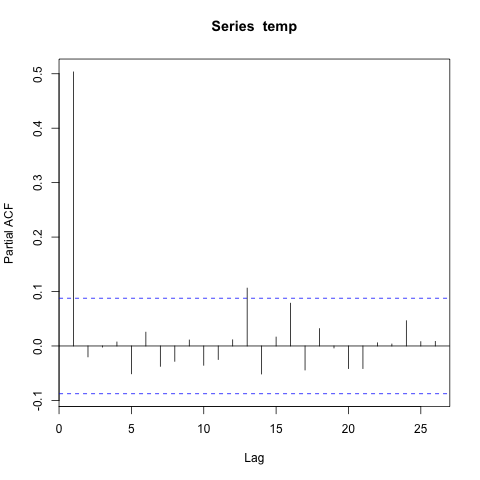
\includegraphics[width=\linewidth]{500-05-pacf}
	\end{subfigure}
	\caption{ACF and PACF plots for $\rho = 0.5$}
\end{figure}


This mirrors the issue motivating this thesis: with short time series, even thought the underlying process has a certain characteristic (in this case, that characteristic is serial correlation in the errors), these characteristics are undetectable with classic tests due to the short length. This first case can be compared to a series of processes with identical lengths, but where $\rho = 0.75$ instead of 0.5. 

\begin{figure}[htp]
	\centering
	\begin{subfigure}{0.23\textwidth}
		\centering
		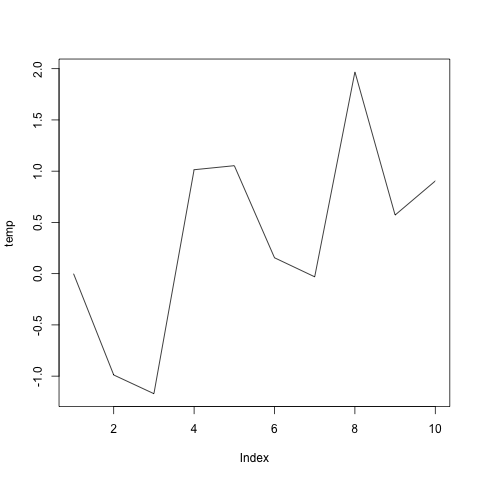
\includegraphics[width= \linewidth]{10-075-plot}
	\end{subfigure}
	\begin{subfigure}{0.23\textwidth}
		\centering
		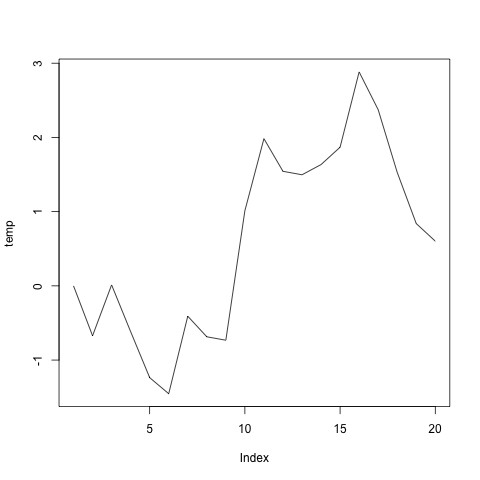
\includegraphics[width=\linewidth]{20-075-plot}
	\end{subfigure}
	\begin{subfigure}{0.23\textwidth}
		\centering
		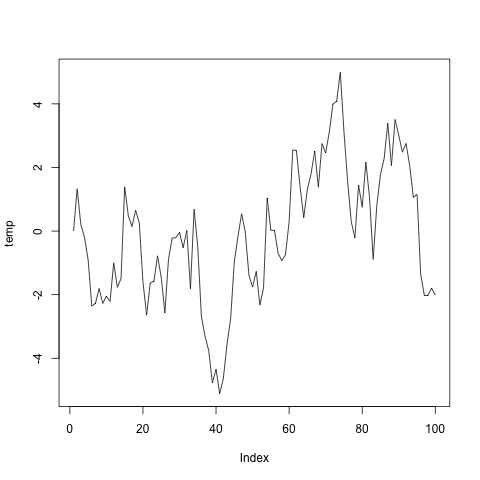
\includegraphics[width= \linewidth]{100-075-plot}
	\end{subfigure}
	\begin{subfigure}{0.23\textwidth}
		\centering
		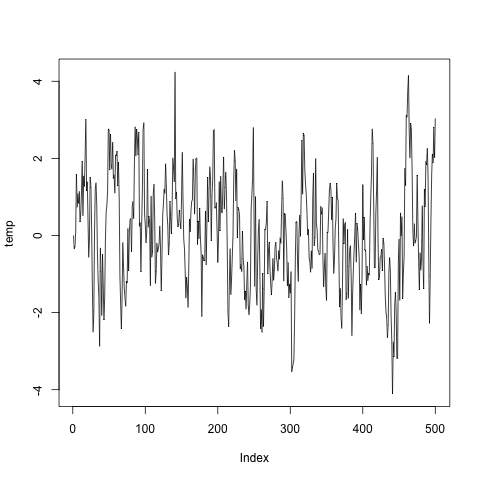
\includegraphics[width=\linewidth]{500-075-plot}
	\end{subfigure}
\caption{Time series plots for $\rho = 0.75$}
\end{figure}



The differences between the two processes are clear, the first process ($T=10$) appears largely stochastic while T = 20 is deterministic with very large residuals. Even $T = 100$ appears to be non-stationary, and it is only when $T = 500$ that the underlying process becomes clear and stationary around a zero mean. The ACF and PACF are likewise different in this case. The ACF for T = 10 does not indicate autocorrelation, but $T = 20$ does slightly so, and $T = 100$ and $T = 500$ exhibit very strong autocorrelation in the ACF. With the PACF behaves similarly, with $T = 10$ indicating no lags, while $T = 20$ indicates (wrongly) an AR(2) process. $T = 100$ and $T = 500$ correctly identify an AR(1) process with the PACF, as is shown below.

\begin{figure}[htp]
	\centering
	\begin{subfigure}{0.23\textwidth}
		\centering
		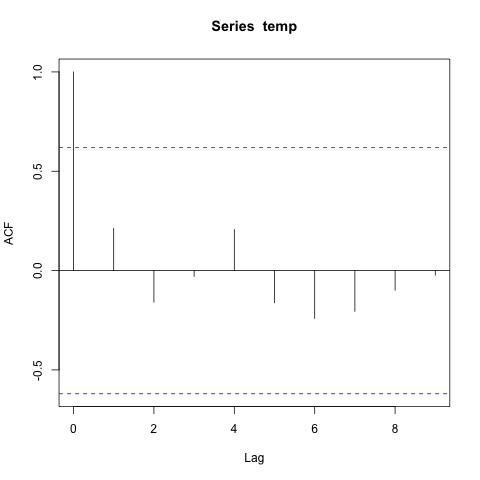
\includegraphics[width= \linewidth]{10-075-acf}
	\end{subfigure}
	\begin{subfigure}{0.23\textwidth}
		\centering
		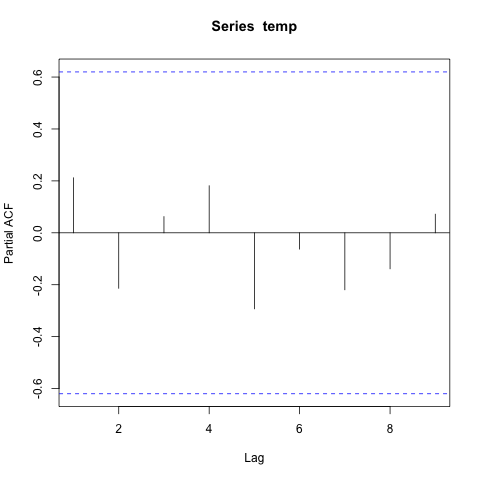
\includegraphics[width=\linewidth]{10-075-pacf}
	\end{subfigure}
	\begin{subfigure}{0.23\textwidth}
		\centering
		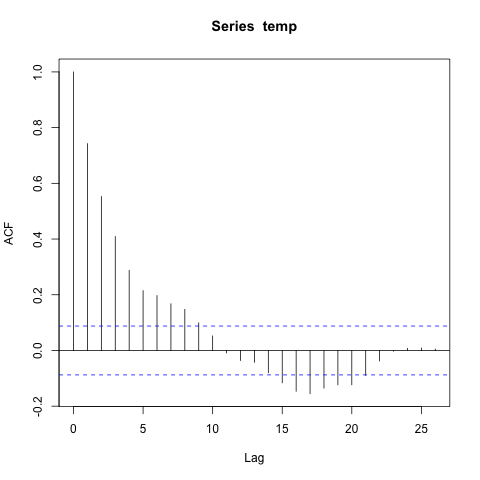
\includegraphics[width= \linewidth]{500-075-acf}
	\end{subfigure}
	\begin{subfigure}{0.23\textwidth}
		\centering
		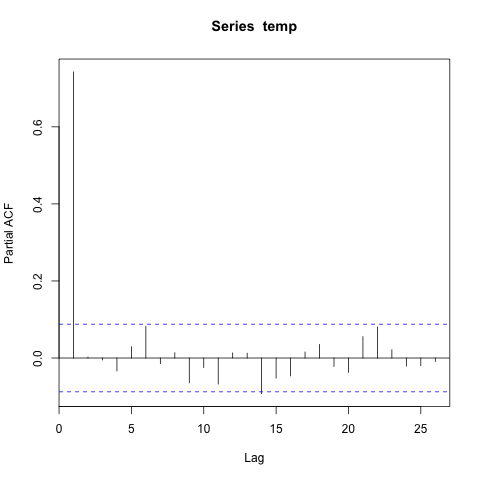
\includegraphics[width=\linewidth]{500-075-pacf}
	\end{subfigure}
\caption{ACF and PACF plots for $\rho = 0.75$}
\end{figure}


Moving further towards a unit root, a process with $\rho = 0.9$ behaves even more stochastically than the previous two processes.

\begin{figure}[htp]
	\centering
	\begin{subfigure}{0.23\textwidth}
		\centering
		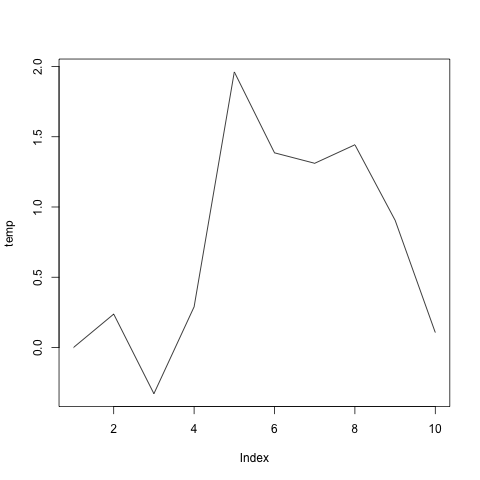
\includegraphics[width= \linewidth]{10-09-plot}
	\end{subfigure}
	\begin{subfigure}{0.23\textwidth}
		\centering
		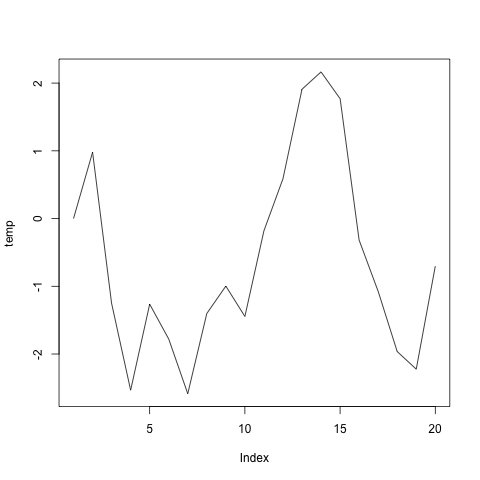
\includegraphics[width=\linewidth]{20-09-plot}
	\end{subfigure}
	\begin{subfigure}{0.23\textwidth}
		\centering
		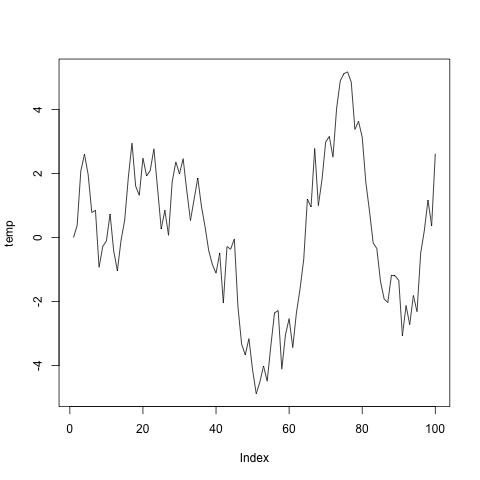
\includegraphics[width= \linewidth]{100-09-plot}
	\end{subfigure}
	\begin{subfigure}{0.23\textwidth}
		\centering
		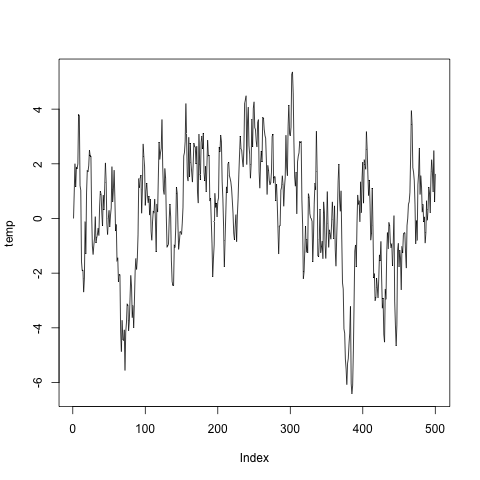
\includegraphics[width=\linewidth]{500-09-plot}
	\end{subfigure}
\caption{Time series plots for $\rho = 0.9$}
\end{figure}


For $T = 10$, $T = 20$ and $T = 100$, the process appears to have a trend while exhibiting a large amount of noise. $T = 500$ beings to resemble a random walk with a drift. None of these are correct diagnoses of the underlying process, however, with remains a zero-mean AR(1) process with an error term, $\epsilon_t$, of $N(0,1)$. The ACF for $T = 10$ is still showing no autocorrelation, while $T = 20$, $T = 100$ and $T = 500$ all show strong autocorrelation. The PACF for this process shows an AR(1) process for all but the shortest series.

\begin{figure}[htp]
	\centering
	\begin{subfigure}{0.23\textwidth}
		\centering
		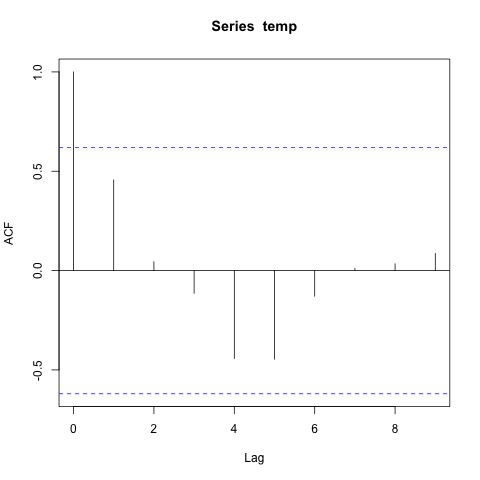
\includegraphics[width= \linewidth]{10-09-acf}
	\end{subfigure}
	\begin{subfigure}{0.23\textwidth}
		\centering
		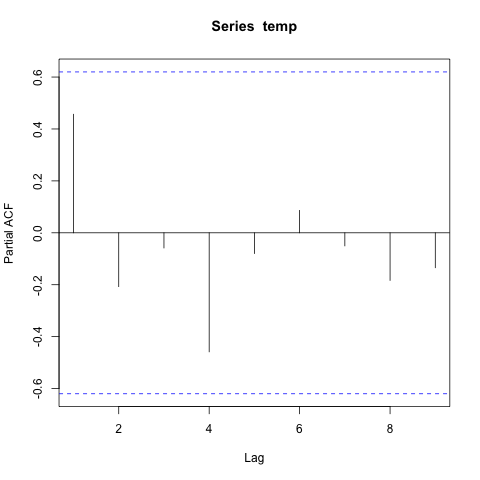
\includegraphics[width=\linewidth]{10-09-pacf}
	\end{subfigure}
	\begin{subfigure}{0.23\textwidth}
		\centering
		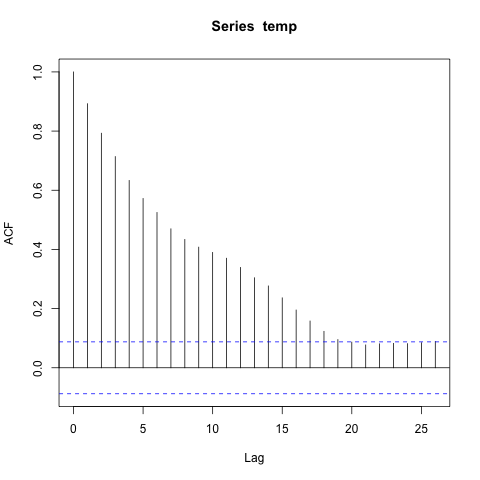
\includegraphics[width= \linewidth]{500-09-acf}
	\end{subfigure}
	\begin{subfigure}{0.23\textwidth}
		\centering
		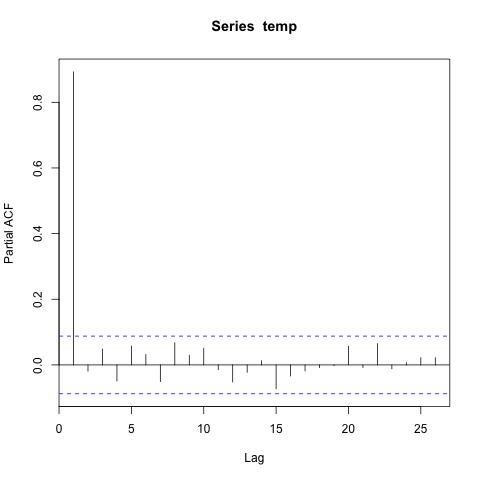
\includegraphics[width=\linewidth]{500-09-pacf}
	\end{subfigure}
	\caption{ACF and PACF plots for $\rho = 0.9$}
\end{figure}


Lastly, it would be prudent to demonstrate a unit root process over the same period of time. It is important to demonstrate the tangible difference between stationary data and non-stationary data in order to motivate the work that follows. The process is effectively a random walk, and this is proven when the process is differentiated, as the deterministic element is eliminated and the only remaining coefficient is the error term, which is a purely stochastic process, hence a random walk:


\begin{equation}
y_t = y_0 + \sum_{i=1}^{T}\epsilon_t
\end{equation}


As is known, a unit root process is an $AR$ process where the $\rho$ coefficient is equal to 1. As demonstrated above, such a process is purely stochastic and thus a random walk.


\begin{figure}[htp]
	\centering
	\begin{subfigure}{0.23\textwidth}
		\centering
		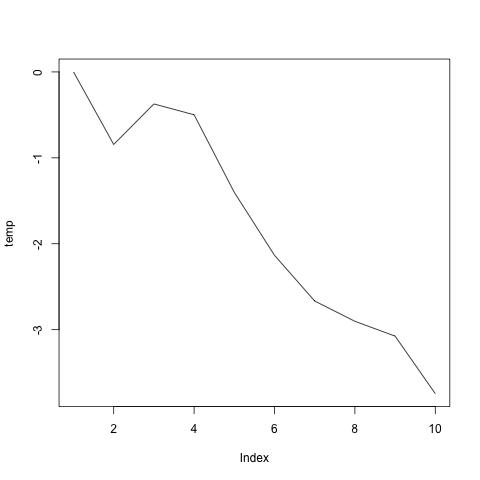
\includegraphics[width= \linewidth]{10-100-plot}
	\end{subfigure}
	\begin{subfigure}{0.23\textwidth}
		\centering
		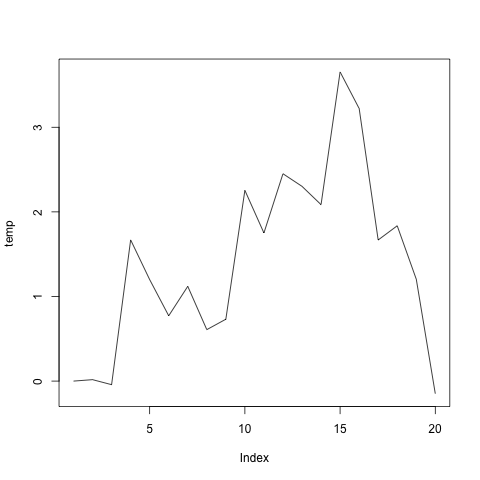
\includegraphics[width=\linewidth]{20-1-plot}
	\end{subfigure}
	\begin{subfigure}{0.23\textwidth}
		\centering
		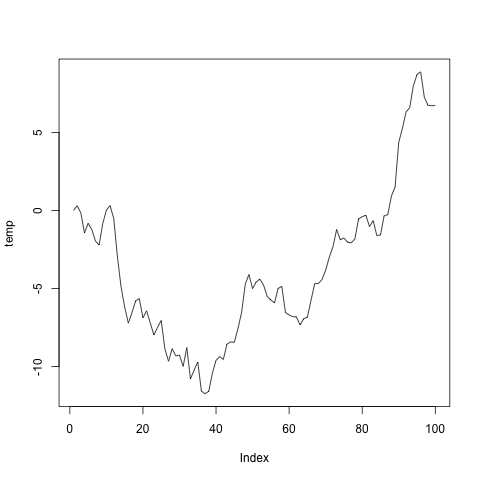
\includegraphics[width= \linewidth]{100-1-plot}
	\end{subfigure}
	\begin{subfigure}{0.23\textwidth}
		\centering
		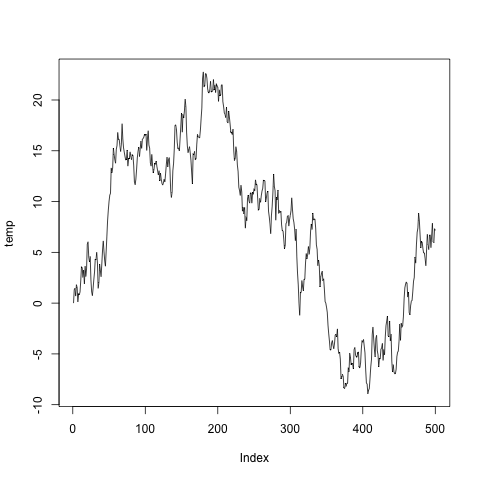
\includegraphics[width=\linewidth]{500-1-plot}
	\end{subfigure}
	\caption{Time Series plots for $\rho = 1$}
\end{figure}


The first interesting thing about the unit root process is that for a short time dimension (say $T = 10$ and $T = 20$), the process appears deterministic, much like the $T = 10$ and $T = 20$ processes of $\rho = 0.75$ and $\rho = 0.9$, which are actually stationary. This is important to note, as this highlights the difficulty faced by stationarity testing for short time series, which will be discussed in detail below. For longer series (say $T = 100$ and $T = 500$), the process is very clearly stochastic, with very abrupt deviations from a short term mean. While the ACF for $T = 10$ did not show autocorrelation (likely because of the small time dimension), $T = 20$, $T =100$ and $T = 500$ all showed a large amount of autocorrelation. When the PACF was used, all but the shortest series showed an $AR(1)$ process with correlations of above 0.8 for the first lag.

\begin{figure}[htp]
	\centering
	\begin{subfigure}{0.23\textwidth}
		\centering
		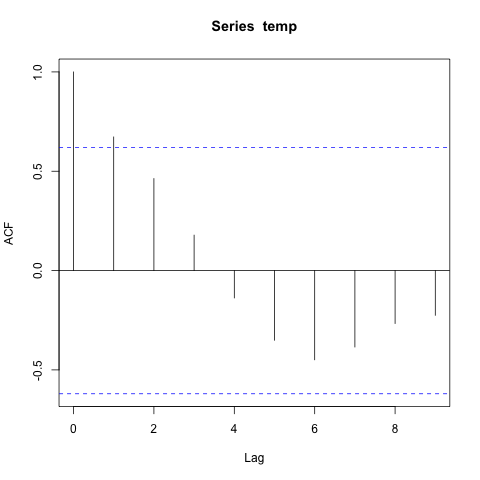
\includegraphics[width= \linewidth]{10-100-acf}
	\end{subfigure}
	\begin{subfigure}{0.23\textwidth}
		\centering
		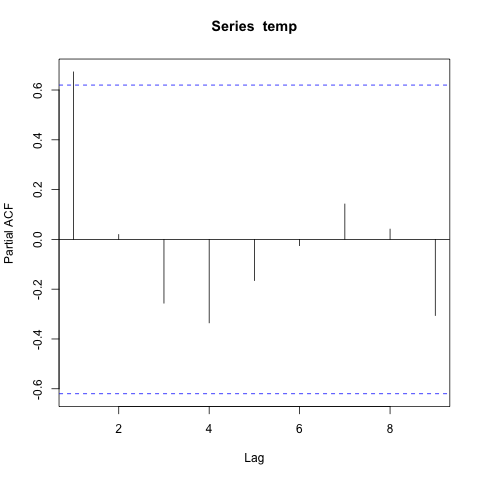
\includegraphics[width=\linewidth]{10-100-pacf}
	\end{subfigure}
	\begin{subfigure}{0.23\textwidth}
		\centering
		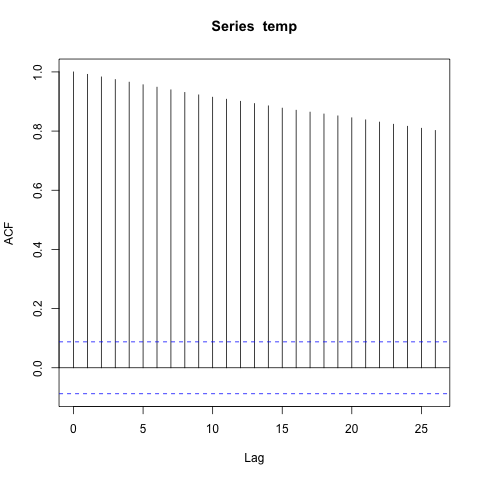
\includegraphics[width= \linewidth]{500-1-acf}
	\end{subfigure}
	\begin{subfigure}{0.23\textwidth}
		\centering
		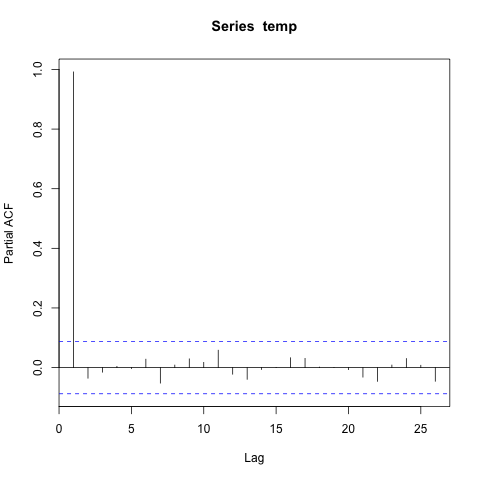
\includegraphics[width=\linewidth]{500-1-pacf}
	\end{subfigure}
	\caption{ACF and PACF for $\rho = 1$}
\end{figure}


Though the underlying process may be stochastic, a short sample of the process examined in isolation may appear and test as a deterministic process. This is visible with the ACF and PACF functions for the shortest series for all cases of $\rho$, where there is clearly not enough data to construct an accurate inference of the underlying data. Visually, the distinction between a stationary and non-stationary process is not large, especially for very short time series. The issue here is that the short dimension of the sample of the process means that the underlying process is not inherently determinable. A similar issue is understandably faced by stationarity testing, where a small sample does not expose enough of the process for correct inferences to be made.

	
	\chapter{Methodology}
	As discussed previously, the methodology is two-fold. The first part involves doing panel unit root tests on a combination of real-world time series, maximising T for every N while maintaining a balanced panel, and comparing the results of these tests with the individual stationarity tests, which will be done on the individuals of each panel. The reasoning behind this is that the panel data tests, with the enhanced cross-section, may offer a higher test power than the individual unit root tests. The second part of the methodology is a Monte Carlo simulation, which will be discussed in greater detail below. Due to errors in the way the Maddala-Wu test was implemented in the software package, additional steps were required to correctly apply it, which are detailed in the final section.

\section{Test Selection}

The choice of tests was limited by two factors. One was software availability; the entire methodology was performed in R, which had a fairly limited choice of panel unit root tests, namely Levin-Lin-Chu 2002, IPS 1997, Hadri 2000, and Maddala Wu 2000. Hadri was ruled out because the null hypothesis is stationarity, as opposed to a null of a unit root with the other three. The remaining tests, the Levin-Lin-Chu and Maddala-Wu, were acceptable due to the fact that the Levin-Lin-Chu is based on the Augmented Dickey-Fuller \citep{said1984testing} approach (therefore is comparable to the ADF test directly) while the Maddala-Wu is designed along the Fisher test principle, which essentially tests each time series in the panel individually, and then transforms the sum of the individual p-values into a test statistic which can be compared to a distribution. The second generation PANIC test was implemented in R, but as that largely depends on the correct specification of the common factors and their loadings, it was decided that the second generation tests would not be comparable to the other tests, and as the remit of this project is a comparison of the existing tests, the PANIC tests would not be included.

The second factor limiting test choice was time. It would take more time than was alloted for this work to create a comprehensive selection of both first-generation and second-generation tests, mostly because the software implementation of many of the panel tests does not exist (at least in the open-source realm, some tests such as the Breitung and Harris-Tzavalis are implemented in professional-grade statistics packages such as SAS) and therefore would have to be created from scratch. Additionally, the Monte Carlo simulations were time intensive to compute as it stood with 3 panel tests and 2 time series tests, therefore the addition of another 3 or so tests would have more than doubled the computation time, which was excessive as it was. Furthermore, the time element was also limited by the corrections required due to the errors with the Maddala-Wu test in the 'plm' package, as is discussed later. The decision to only use the Levin-Lin-Chu, Im-Pesaran-Shin and Maddala-Wu was therefore well justified.


For single time series unit root tests, the only real candidates were the Augmented Dickey-Fuller and the Phillips Perron. The KPSS test was considered initially, however the fact that the null and alternative hypotheses were different from the ADF and PP (KPSS has a null that the series is stationary vs. non-stationarity) meant that the KPSS was ruled out. ADF and PP have slightly different specification in that ADF is robust to deal with different AR and MA orders while PP is not, but this was not an issue, as the lag order was determined manually prior to using the tests, as was described in the data section. The ACF and PACF plots of each time series were examined and a decision was made to consider the data $AR(1)$.

The procedure for the Augmented Dickey Fuller was straightforward. Once the lag order was selected, the difference of the series (denoted as $\Delta y_t$) was regressed upon the lagged series (denoted as $y_{t-1}$) and the lagged difference of the series (denoted as $\Delta y_{t-1}$). The resulting critical value for the lagged series was compared with the Dickey-Fuller distribution based on the form of the DGP, which in this case was zero-mean, and if the critical value generated was less than the value given in the distribution, the null hypothesis was rejected in favour of the alternative, and the series is considered stationary.

The Phillips-Perron procedure is identical to the Augmented Dickey-Fuller test, except for the way that serial correlation is dealt with. While the ADF test adds the appropriate amount of lags to the final regression before the test statistic is generated, PP corrects the test statistic from the initial regression to correct for the presence of serial correlation.

The single time-series stationarity tests were sourced from the “tseries” package while the panel data stationarity tests were performed using the "plm" package, the full details and credits for both of these packages are given in the appendix. A few notes on the specification of the tests: the p-max variable, given in the tests to determine the maximum lag for which the significance should be tested, as described in $\cite{said1984testing}$, was set to 1 as this was determined to be the lag order when the data was being tested for auto-correlation. This also served to eliminate any advantage a particular test might have due to a superior lag-selection procedure. The exogenous variables were set to trend, as the data was identified as following a trend with intercept pattern in the data chapter (specifying 'trend' in the test function automatically added an intercept as well).

\section{Procedure}

The first step was to create panels from the individual time series. The panel sizes ranged from 39 observations of 2 individuals to 8 observations of 36 individuals. For each panel created, the two selected time series stationarity Augmented Dickey-Fuller and Phillips-Perron) tests were run on each individual time series, followed by the three selected panel data stationarity tests. The reason for this is to have direct comparability between the individual tests and the panel tests. The code for this is located in the appendices and discussed there in greater detail.

\section{Simulation}

For the simulation part of this investigation, panels were algorithmically generated in a range of predefined sizes, ranging from 2 to 50 for the individual dimension and 8 to 25 for the time dimension. The panels were comprised of autoregressive processing of order one (AR(1)), and the $\rho$ coefficient varied depending on the case being investigated. As stated in the data section, the coefficients for $\rho$ varied from 0.5, 0,75, 0.9, 1 where all but the last coefficient were stationary processes. The processes were all trend and intercept processes and can be expressed by:

\begin{equation}
y_t = \alpha + \beta t + \rho y_{t-1}
\end{equation}

Once each panel was generated, an ADF test and a PP test were performed on each individual in the panel, and the results were saved. Once this was completed, the panel unit root tests were performed, specifically the Levin-Lin-Chu and the Maddala-Wu. The procedures for both are described in more detail in the Literature Review section but will be mentioned here shortly. The LLC test performs the ADF on each individual and saves both sets of residuals, say $\bar{e}$ and $\bar{f}$. $\bar{e}$ is then regressed on $\bar{f}$, and the standard error from this regression is used to standardize $\bar{e}$ and $\bar{f}$ into $\hat{e}$ and $\hat{f}$. Following this, both long-run and short-run variance is calculated and then the test statistic is calculated using the formula mentioned in 2.3.1 under "Levin et al 2002." This statistic is then compared to the correct distribution, which is normal for zero-mean cases and has to be normalized for either an intercept or trend case.


The Maddala-Wu is by comparison much more straightforward: each individual time series undergoes an individual unit root test, which can be any test desired (in the "plm" package the chosen test is the Augmented Dickey-Fuller), and the p-values of these tests are saved. The p-values are then passed through the formula mentioned in 2.3.1 to generate a test statistic which follows a chi-squared distribution with 2*N degrees of freedom. 

The Im-Pesaran-Shin is very similar to the Maddala-Wu test in that it is averaging the results from individual tests. Unlike the Maddala-Wu, however, the Im-Pesaran-Shin test takes the critical value generated from the Dickey-Fuller regression and averages it, generating a test statistic which is then standardized and is normally distributed as $T \to \inf$ and $N \to \inf$.

\subsection{Software}

Because each process in each panel had a stochastic element (the error term) the simulation was a Monte Carlo simulation with 10,000 iterations for each dimension, and for each iteration the individual tests would be done on the individuals, followed by the panel data test, but the underlying panel data would not change during the iteration.

In terms of software, while this will be discussed somewhat in the appendix, it should be noted that this investigation relied heavily upon pre-programmed libraries available for R, as the time frame was too short to develop bespoke and robust testing procedures. The libraries which were used were “plm” and “tseries” for the tests, as well as the “parallels” and “foreach” libraries”, each of which had their own dependacies which are listed fully in the appendix. “Parallels” and “foreach” were used for their parallel computation, as the Monte Carlo simulations were extremely computation-intensive, requiring over 8 billion instances were a panel was created and tested. The details of these packages is included in the appendix.

\section{Maddala-Wu Implementation}

The implementation of the Maddala-Wu panel test in the "plm" library uses the Augmented Dickey-Fuller test as the individual test, from which the p-values are then sourced. The issue with the implementation is that after the critical values are calculated, they are then compared to a normal distribution to determine the p-values. As is known, the critical value in the Dickey-Fuller test must be compared to a bespoke Dickey-Fuller distribution, which will depend on the case (zero-mean, intercept, or trend) and the length of the series. The way that this issue was overcome was that the Dickey-Fuller distributions were created using Monte-Carlo simulations, and the critical values were generated from a bespoke Augmented Dickey-Fuller test and compared to the custom distributions. The code for steps described is located in the appendix.





	
	\chapter{Results}
	\section{Results Overview}

\subsection{Real Data}
\begin{figure}[htp]
	\centering
	\begin{subfigure}{0.3\textwidth}
		\centering
		\begin{lstlisting}[language=R,basicstyle=\tiny]
		
Levin-Lin-Chu Test
Stationary:     27
Non-stationary: 8

		\end{lstlisting}
	\end{subfigure}
\begin{subfigure}{0.3\textwidth}
	\centering
	\begin{lstlisting}[language=R,basicstyle=\tiny]

Maddala-Wu Test
Stationary:     7
Non-stationary: 28

	\end{lstlisting}
\end{subfigure}
\begin{subfigure}{0.3\textwidth}
	\centering
	\begin{lstlisting}[language=R,basicstyle=\tiny]

IPS Test
Stationary:     22
Non-stationary: 13

	\end{lstlisting}
\end{subfigure}

\caption{Summary of Panel Test results.}
\end{figure}


The results in Figure 5.1 clearly show that the Levin-Lin-Chu test strongly rejects the null hypothesis of the data following a unit root majority of the time. There are a few cases where the tests results indicate that the panels are not stationary, but these are instances where the panel dimensions are $N \to 0$ and $T \to \inf$. The IPS test results indicate stationarity in the panels as a whole, but a larger minority of non-stationary results was present here than in the Levin-Lin-Chu or Maddala-Wu. By contrast, the individual tests (results shown in Figure 2), the Augmented Dickey Fuller and Phillips-Perron, both overwhelmingly state that most of the time series they test are not stationary. An interesting characteristic of the data is that the test statistic of the individual unit root tests changed by a relatively large degree when single observations were removed, which suggests that the tests were not robust to small sample sizes.

\begin{figure}[htp]
	\centering
	\begin{lstlisting}[language=R]
	===============
	Summary Results
	===============
	ADF Test
	Stationary: 2   Non-Stationary: 34
	PP Test
	Stationary: 0   Non-Stationary: 36
	\end{lstlisting}
	\caption{Results of individual tests}
\end{figure}



\subsection{Simulated Data}

The results of the simulations were re-arranged into graphs where the x-axis was the time dimension, increasing to the right, the y-axis was the individual dimension, ascending, and the colours correspond to the average p-value generated, with green being at or below 0.01, yellow is 0.05 and red is 0.1 and above.

\begin{figure}[htp]
	\centering
	\begin{subfigure}{0.3\textwidth}
		\centering
		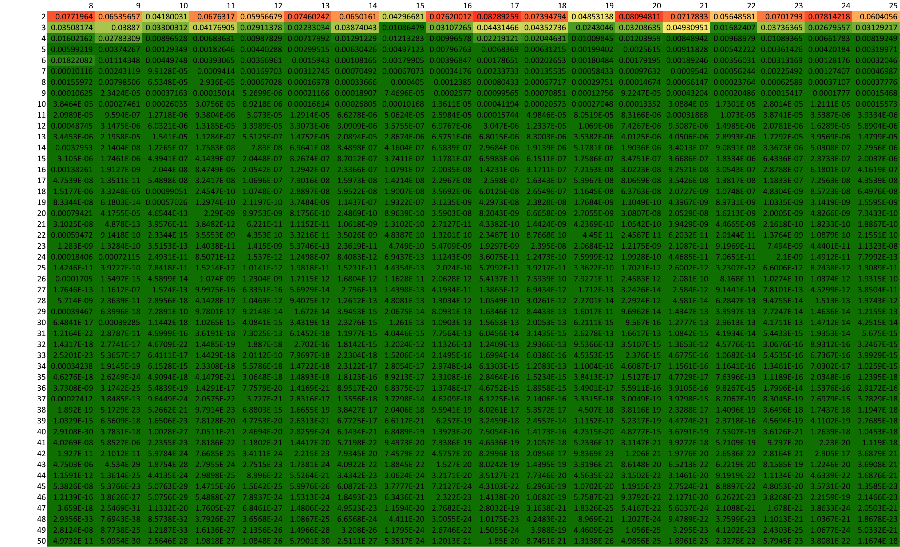
\includegraphics[width= \linewidth]{llc-050}
	\end{subfigure}
	\begin{subfigure}{0.3\textwidth}
	\centering
	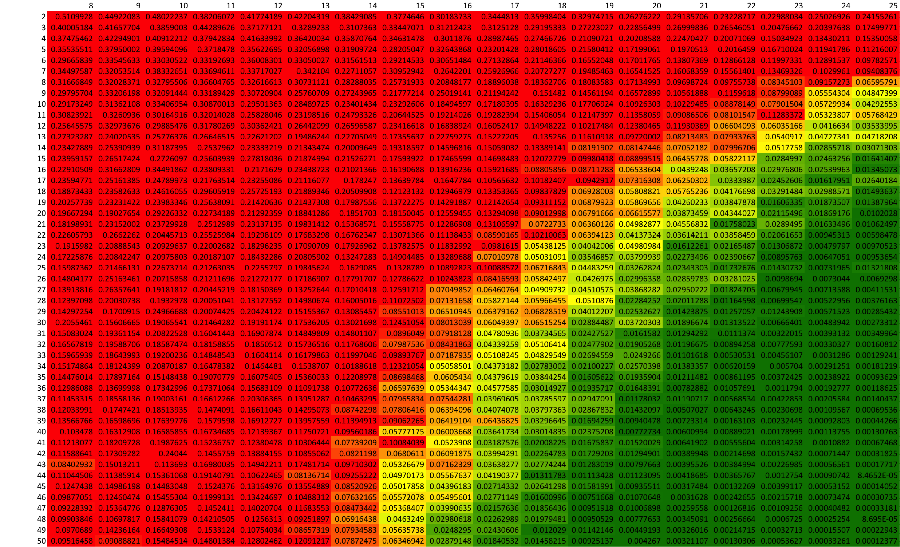
\includegraphics[width= \linewidth]{mw-050}
\end{subfigure}
	\begin{subfigure}{0.3\textwidth}
	\centering
	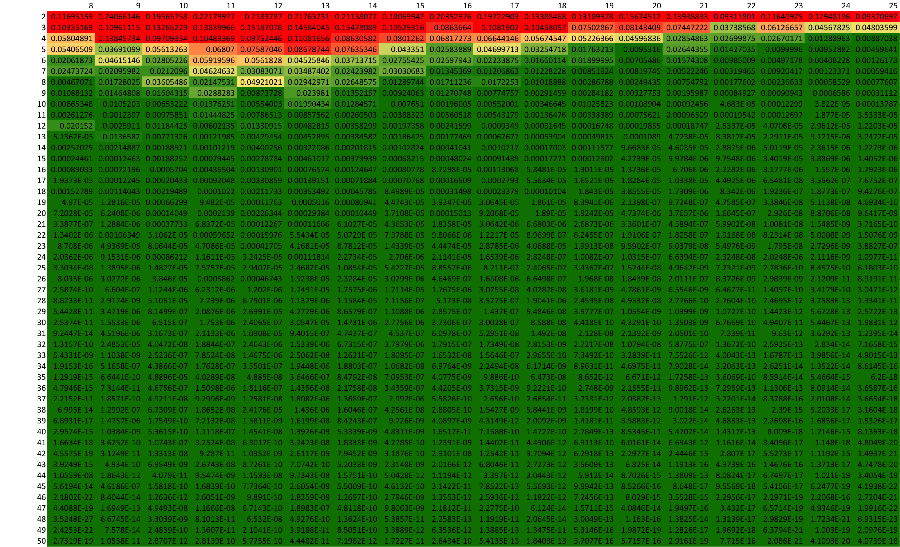
\includegraphics[width= \linewidth]{ips-050}
\end{subfigure}
\caption{Results for the Levin-Lin-Chi, Maddala-Wu and IPS when $\rho = 0.5$ (from left to right)}
%\subcaption{Note: the x-axis is T and the y-axis is N}
\end{figure}
%Note: In this section, I would include heat-maps with the 

The simulations initially seemed to show the Maddala-Wu performing better than the Levin-Lin-Chu when it came to correctly identifying datasets with $\rho$ less than but very close to 1, meaning they were on the verge of having a unit root. However, this was discovered to be due to the programming error discussed in Chapter 4, and the real results for the Maddala-Wu showed an overwhelming tendancy to fail to reject the null hypothesis. The IPS, on the other hand, appeared to perform comparably to the Levin-Lin-Chu at $\rho = 0.5$. When compared to the Levin-Lin-Chu, the Maddala-Wu was quicker to move away from rejection territory as $\rho \to 1$, but the IPS moved further from rejection territory as the $T \to \infty$. With that said,both the Levin-Lin-Chu and IPS seemed be accurate at rejecting the null when $\rho = 0.5$.

\begin{figure}[htp]
	\centering
	\begin{subfigure}{0.3\textwidth}
		\centering
		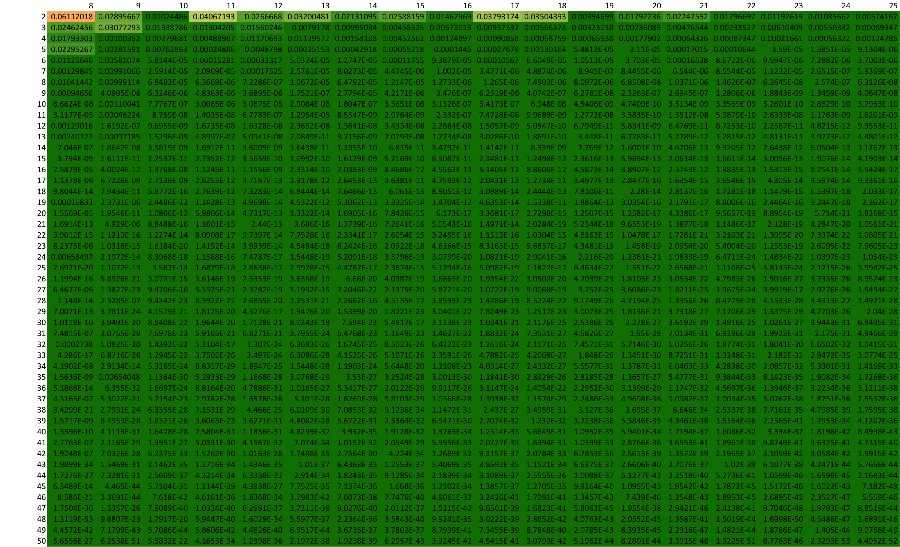
\includegraphics[width= \linewidth]{llc-075}
	\end{subfigure}
	\begin{subfigure}{0.3\textwidth}
		\centering
		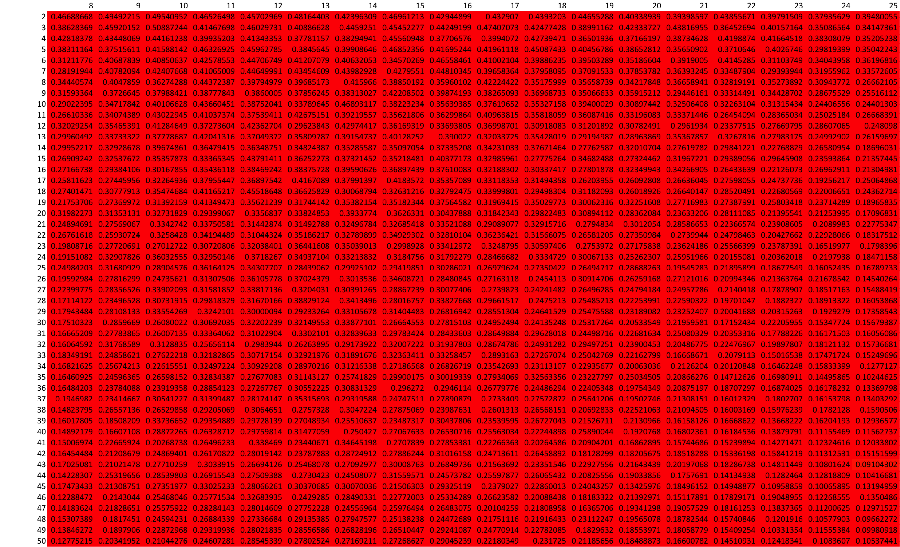
\includegraphics[width= \linewidth]{mw-075}
	\end{subfigure}
	\begin{subfigure}{0.3\textwidth}
		\centering
		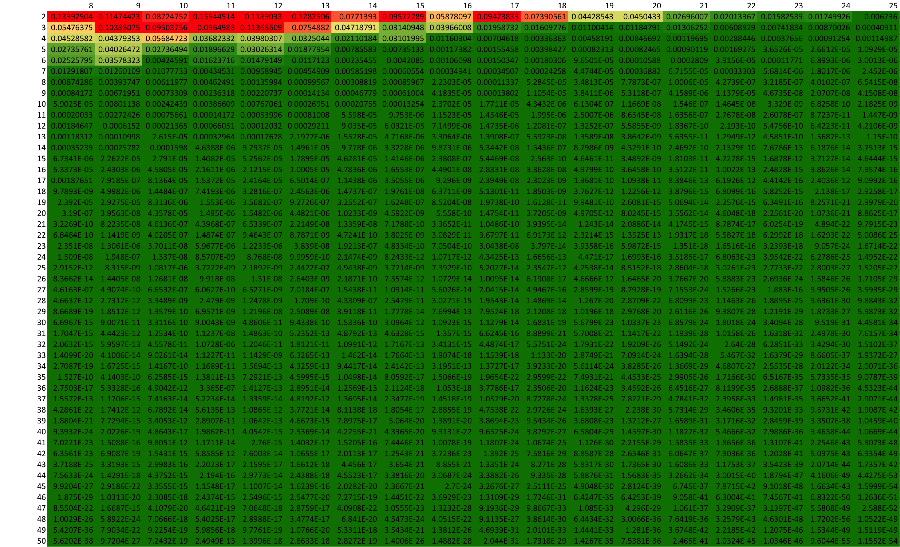
\includegraphics[width= \linewidth]{ips-075}
	\end{subfigure}
	\caption{Results for the Levin-Lin-Chi, Maddala-Wu and IPS when $\rho = 0.75$ (from left to right)}
	%\subcaption{Note: the x-axis is T and the y-axis is N}
\end{figure}

Moving to the case of $\rho = 0.75$, the Levin-Lin-Chu and IPS performed nearly identically with regards to rejecting the null and panel dimensions as with the previous case. The Maddala-Wu, on the other hand, wholly failed to reject the null on average for all panel dimensions tests for $\rho = 0.75$ as well as $\rho = 0.9$ and $\rho = 1$.

\begin{figure}[htp]
	\centering
	\begin{subfigure}{0.3\textwidth}
		\centering
		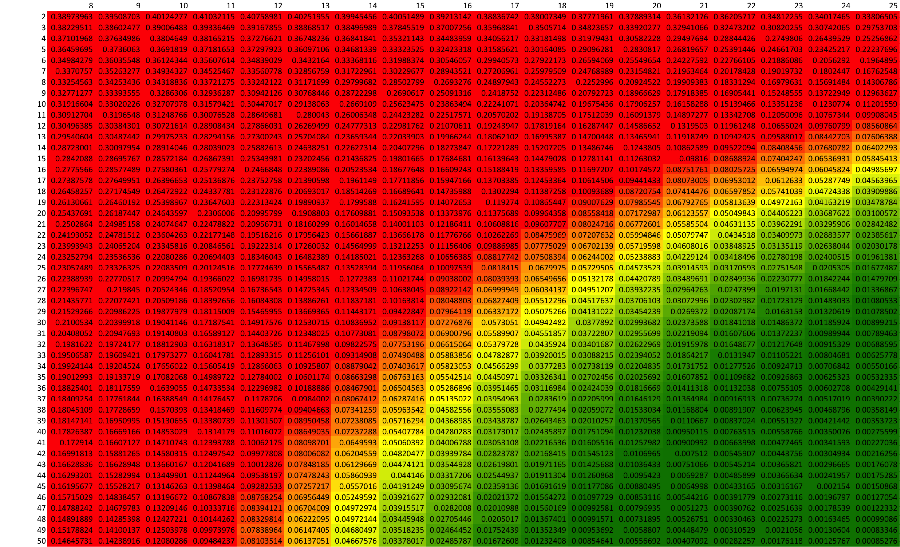
\includegraphics[width= \linewidth]{llc-090}
	\end{subfigure}
	\begin{subfigure}{0.3\textwidth}
		\centering
		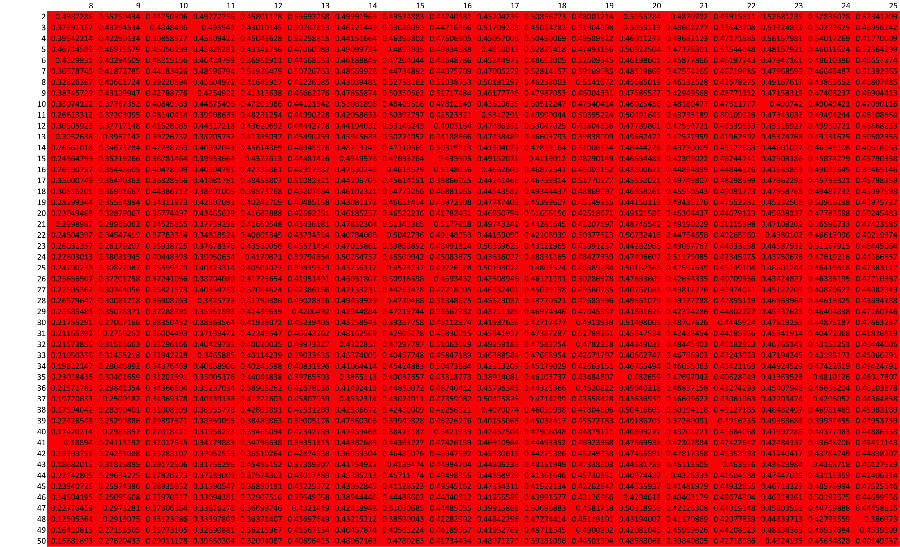
\includegraphics[width= \linewidth]{mw-090}
	\end{subfigure}
	\begin{subfigure}{0.3\textwidth}
		\centering
		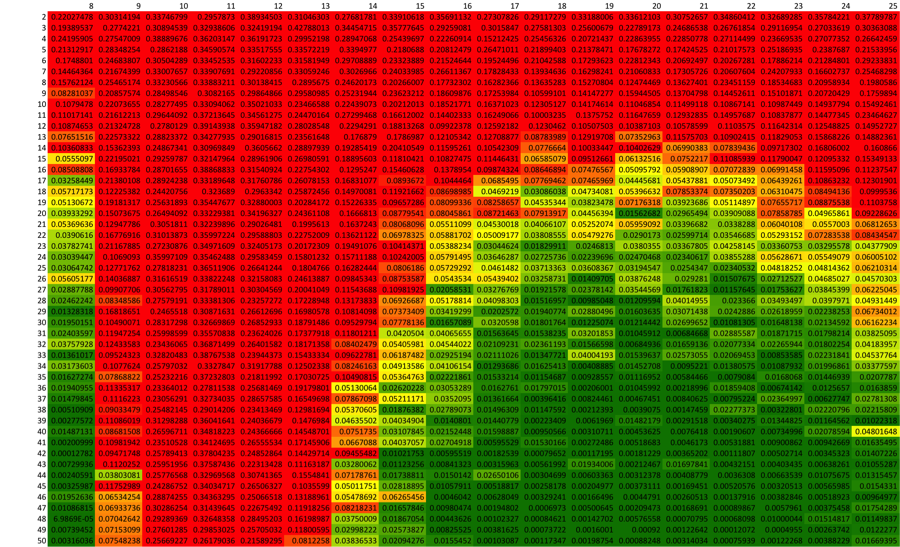
\includegraphics[width= \linewidth]{ips-090}
	\end{subfigure}
	\caption{Results for the Levin-Lin-Chi, Maddala-Wu and IPS when $\rho = 0.9$ (from left to right)}
	%\subcaption{Note: the x-axis is T and the y-axis is N}
\end{figure}


The case of $\rho = 0.9$ began to show more of the relationship between the panel dimensions and null rejection. The Levin-Lin-Chu demonstrated that as $N$ and $T \to \infty$, the power of the test increases and it moves away from Type I errors, where the null hypothesis is wrongly not rejected. The Maddala-Wu, as stated previously, continued to demonstrate complete failure to reject the null hypothesis. The Im-Persaran-Shin test began to exhibit an odd trait, however, as there appeared to not be as clear a relationship between panel dimensions and p-values, at least not a linear one. This curiosity continued in the subsequent test, albeit to a lesser degree.

\begin{figure}[htp]
	\centering
	\begin{subfigure}{0.3\textwidth}
		\centering
		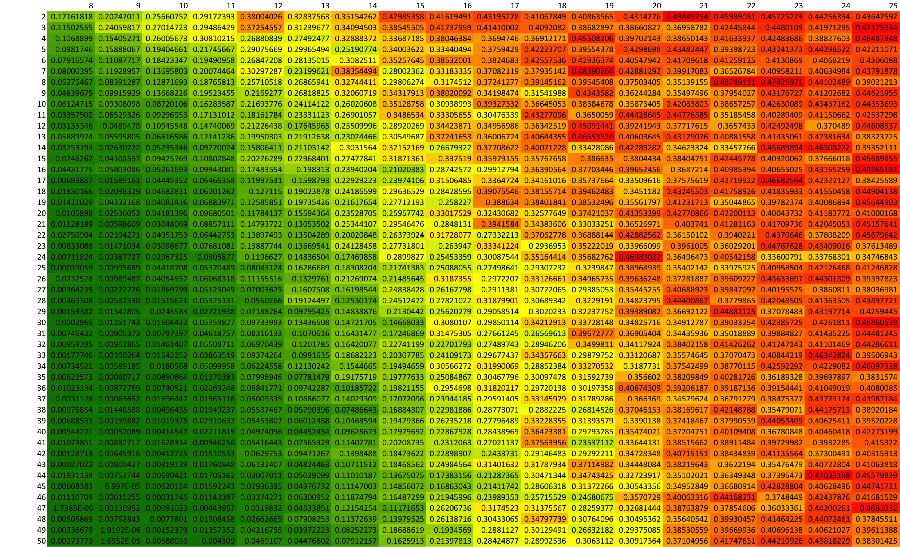
\includegraphics[width= \linewidth]{llc-100}
	\end{subfigure}
	\begin{subfigure}{0.3\textwidth}
		\centering
		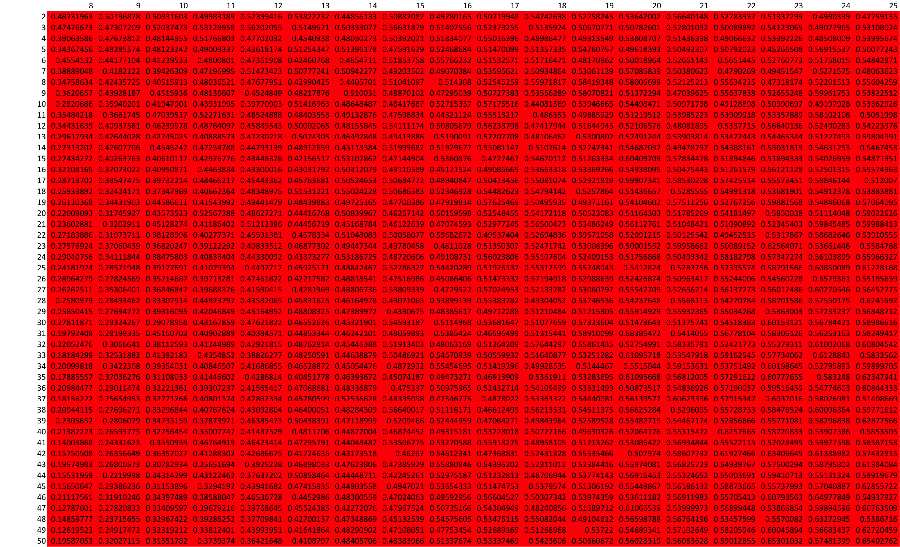
\includegraphics[width= \linewidth]{mw-100}
	\end{subfigure}
	\begin{subfigure}{0.3\textwidth}
		\centering
		\includegraphics[width= \linewidth]{ips-100}
	\end{subfigure}
	\caption{Results for the Levin-Lin-Chi, Maddala-Wu and IPS when $\rho = 1$ (from left to right)}
	%\subcaption{Note: the x-axis is T and the y-axis is N}
\end{figure}

The final case which was examined was the case of a unit root, or where $\rho = 1$. The most notable result here was the Levin-Lin-Chu test, which appeared to reverse its relationship with the dimensions of the panel. As the panel increased in size, the Levin-Lin-Chu test was less likely to reject the null hypothesis of a unit root. The Maddala-Wu performed identically to the way it had in the previous cases. The Im-Persaran-Shin, however, began to have a more linear relationship with the dimensions of the panel, albeit with the small tendency to reject the null for cases where $N$ was high but $T$ was low.

\section{Analysis}

\subsection{Real Data}

The panel unit root tests done on the real data overwhelmingly rejected the null hypothesis of a unit root (with the exception of the Maddala-Wu), while the time series tests very quickly began to fail to reject the null hypothesis of a unit root as the time series dimension fell. The key question with the real data is whether the results are spurious or have actual value. As noted above, the individual tests did not show consistency, significantly changing the critical value from rejection territory to non-rejection territory with only one observation removed and vice versa. This exemplifies the criticism often levied at single time series stationarity tests, in that for time series with a small number of observations (below 100), the tests have extremely limited power, meaning that even if the single stationarity test indicated a time series was correctly stationary, the result was most likely spurious and coincidental. It is important to note how the panel unit root tests behaved when the time series dimension was large but the individual dimension was low. The panel tests tended to show that the panels were not stationary, but it is important to view these results in light of the Monte Carlo simulations. In the MC simulations, it was shown that the tests quickly converge to a p-value as individual dimensions are added, while the initial p-value is quite high for an individual dimension of 2 or 3 (therefore failing to reject the null of a unit root). It therefore follows that the tests have a power similar to that of single time series tests (such as the ADF or PP) for cases where the individual dimension was small, such that it was for the first few instances of the real data which were tested (i.e. a panel test on data consisting of 50 observations of 2 individuals will perform very similarly to a single time series). Indeed, one recommendation in \citet{llc} was that for instances where $N \to 0$, but the time series dimension was large, the panel data stationarity tests had similar power to single time series unit root tests, which themselves had low power in cases where the series was short, which was also the case for the panels tested. The results for the real data tests in this paper are therefore consistent with the literature discussed previously.

\subsection{Simulated Data}


The key take-away from the Monte Carlo simulations is that the tests generally responded to changes in dimensions, albeit in different manners. The LLC test appeared to gain power exponentially as either the time or the individual dimension increased. The Maddala-Wu test exhibited the same kind of relationship between the p-value generated and the dimension of the panel as the Levin-Lin-Chu, but appeared to be more sensitive to the auto-regressive coefficient. A likely explanation of this is due to the fact that the Maddala-Wu is a Fischer-style test $\citep{fisher}$, it involves pooled test statistics of individual tests, which are acknowledged to have low power for short time series, which caused great variability between components of the panel when tested individually. As the time series component of the panels grew, so did the power of the Maddala-Wu test, as is visible in the first case where $\rho = 0.5$. By contrast, the Levin-Lin-Chu appeared to be robust to either extreme, and for all values of $\rho$ tested, the dimension appeared to be a very important factor in the power of the test, as indicated by the heatmaps generated. Comparatively, the heatmaps for the Maddala-Wu show that as the value of $\rho$ grows (i.e. the underlying process is closer to being a non-stationary process) the test overwhelmingly indicates that the panel contains a unit root. The Im-Pesaran-Shin test, on the other hand, performed very poorly, compared to the two previous tests. The behaviour of the p-values with respect to the time and individual dimensions did not appear to follow a strict linear trend. For the last two cases, the test started with relatively low p-values, moving up further from rejection territory, only to level out and then begin descending as the time dimension grew. The problem appears to subside with the unit-root case, but there the test wrongly moves to reject the null as the panel grows in size. The Maddala-Wu appears to have a relationship between its power and the size of the panel, but is much too sensitive to be of use for panels of the sizes tested. By contrast, Levin-Lin-Chu strongly fails to reject the hypothesis, which is desirable for the unit-root case. In addition, the Levin-Lin-Chu does not converge as strongly to a low p-value in the unit-root case, and does not converge to acceptance level at 10\% significance above 16 observations and a large cross-section (at least 50) for the unit root case.

A point discussed in the literature review was the fact that the traditional unit root tests for single time series lacked power for small time series, and this was confirmed with the Monte Carlo simulations. Even for simulations with relatively small rho values, the ADF and PP tests consistently returned a non-rejection p-value when in fact the null should have been rejected. While the panel tests performed similarly when the individual dimension was small, the advantage of pooling data in the panel data format and applying panel data unit root tests is quite clear. With an increasing individual dimension, the Levin-Lin-Chu test gains power to quickly converge at a consistent mean p-value, suggesting a saturation point where increasing the individual dimension sees diminishing marginal returns in test power. This means that there exists a minimum individual dimension which could guarantee some minimum reliable test power. This is consistent with the literature mentioned $\cite{baltagi2001nonstationary}$, where the effect of adding an individual dimension is statistically akin to additional sampling of the same distribution. It is valid, therefore, to conclude that the combination panel tests (such as the Maddala-Wu and Im-Persaran-Shin) are not as powerful with small panels as the Levin-Lin-Chu test is.


\section{Summary}

The goal was to demonstrate that with a data generating process following AR1, a $\rho$ value of < 1 would be more detectable with the panel data format, even if neither the time nor individual dimensions were generous. This has been achieved, with the panel data tests being robust to relatively high values of rho, especially when compared to single time series tests. In cases where the individual dimension stayed small but $T \to \inf$, the test power of the individual time series tests converged to that of the panel data tests.

The conclusion to draw from the results of the Monte Carlo simulations is that the Levin-Lin-Chu panel data test performs remarkably better in situations where the time series dimension is limited, but the individual dimension is generous. The MW test appears to perform well in cases where the $\rho$ coefficient is small, but has limited power as it increases. The Im-Pesaran-Shin did not exhibit a rational relationship between test power and panel dimensions. One conclusion which could be drawn from this is that the Maddala-Wu test has a tendency to produce type II errors with panels of large auto-regressive coefficients. The Levin-Lin-Chu test, on the other hand, is more likely to produce type II errors when the T and N dimensions are small, but at around 15 observations of 30 individuals the test rapidly converges to acceptance level p-values. The IPS must be ruled out of consideration as a test for small panel sizes, as the performance in the Monte Carlo simulations didn’t indicate a consistent relationship between panel size and test power, which may suggest a similar error in programming as was evident in the Maddala-Wu. An important point to make with all the tests is that the power is severely lacking for instances where the panel has a low T and N dimension. As mentioned by literature, however, the essence of panel data tests is to increase test power in situations where the time dimension is limited. And when comparing the Maddala-Wu and Levin-Lin-Chu, the former does move into rejection territory as $N \to \inf$, but this is often of the type I variety, while the Levin-Lin-Chu is more likely to reduce type II as $N \to \inf$ without moving into error type I territory. This discrepancy in the performance of the tests is down to the way they are specified. The Maddala-Wu pools p-values of individual time series unit root tests, which have been noted to have very low power when the T value is small, therefore the Maddala-Wu test pools low-power statistics together leading to a low-power panel data test when the T value is small. The Imp-Persaran-Shin does a similar task, except that instead of pooling p-values, it pools critical values, which has been shown to be even worse as a method than with the Maddala-Wu. The Levin-Lin-Chu, on the other hand, saves residuals and then regresses them on each other, creating one pooled statistic. In this sense, it takes more advantage of the cross-sectional dimensional nature of the data, which is why the test has more power than the Maddala-Wu or the Im-Pesaran-Shin, who both use a derivative of the Fisher method. For cases with medium-sized T dimension but a large N dimension, the Fisher method may result in a more powerful test, but for cases with very limited T but large N dimensions, the Maddala-Wu and Im-Pesaran-Shin are taking p-values and critical values of already severely weak tests, ergo the resulting statistic will be flawed at best and completely wrong at worst.


	
	\chapter{Evaluation}
	\section{Review of Work}

\subsection{Intention}
This work’s aim was two-fold: perform panel data unit root tests on real-world data and determine which of the panel data tests perform better under which conditions. In regards to the first aim, this project succeeded. The given data was tested both with single time series unit root tests and panel data unit root tests, and it was found that while the single time series tests largely indicated that all the series were non-stationary, as the individual dimension of the panels grew, the panel unit root tests increasingly found that the panels were stationary.

In terms of the simulations, panels of varying dimensions were created, tested individually and then subjected to panel unit root tests in a Monte Carlo simulation, where each iteration of the simulation involved creating a new time series using the same process. All the panel data tests were found to react to the changes in dimension by way of either reduced or increased power. The panels where both T and N were large produced less type I errors and type II errors. When T and N were not large, the panels would always fail to reject the null, but as the dimensions were slowly increased, the rate of change in the p-value produced by the tests varied from test to test. It was found that the Levin-Lin-Chu had the most desirable performance, while the Maddala-Wu tended towards type I errors and the Im-Perasan-Shin did not behave in an explicable way as the dimensions were increased. 

But how to interpret these results? The first step is to generate an understanding of the relationship between the test results and the characteristics of the input data. It appears that Fisher-type tests, which are simply an aggregation of p-values from individual tests, are far too likely to pronounce a panel as unstationary, even when the underlying process of the individual time series is a deterministic process. This means that if the Maddala-Wu was relied upon to test real-world data, the inferences formed on all subsequent tests done on the panel would be flawed, because nearly all meaningful statistical inferences require the data to be at least trend stationary. The Im-Pesaran-Shin, which is inspired by the Fisher-type tests except that critical values are averaged out instead of p-values, performed even worse.

\subsection{Flaws With Methodology}

A way to improve on the methodology in this thesis is to increase the number of panel unit root tests which were run. Due to software and time limitations, this work relied upon external libraries to supply panel data unit root tests. Given that these tests are a relatively new field, especially those which account for cross-sectional dependence, it is understandable that they would not be readily available to use in pre-programmed form. What is less understandable, however, is the fact that a test was implemented incorrectly, attempting to use a normal distribution to interpret a Dickey-Fuller statistic. Having said that, it would not take a great deal of time to create a robust package which facilitated these tests (robust here meaning that the package would be able to deal with all the nuances expected of software packages, such as error reporting, dealing with different input data types, etc), just more time than was afforded to this thesis. As a result, this work merely opened the door to question posed by it.


Another issue with the work was that some time was spent correcting issues with the pre-existing packages. Notably, the implementation of the Maddala-Wu test in the "plm" package was incorrect. As was discussed in Chapter 2, the Maddala-Wu is a Fisher-type test, which in the way it was implemented in R tested each individual with the Augmented Dickey-Fuller test, generated p-values and then applied the formula 2.10 in order to generate the t-statistic. The issue with this implementation is two-fold: the calculation of the p-values and the input limitations. The p-values were calculated by looking up the critical value on a normal distribution, but $\cite{df}$ clearly state that there is a specific Dickey-Fuller distribution which is to be used. As a result, the p-values generated by the test are invalid. In addition, the implementation of the test required that the input data be in a balanced format, which is not required in the actual test as detailed by $\cite{mw}$. The way that this was resolved, however, was that a custom version of the test was developed, which compared the critical values against Dickey-Fuller distributions that were manually generated through a Monte Carlo simulation. This corrected for the p-values. The second problem is more to do with the R programming language conventions, where the Data-Frame, the conventional way of storing panels, cannot by definition be unbalanced. This was not actually an issue in the implementation of the methodology, as this created balanced panels to ensure comparability with other panel data tests which require balanced panels in the literature. Furthermore, an easy way to overcome the Data-Frame limitation is to manually balance the panels by introducing "NA" variables for the shorter individuals until the panel is balanced.




One way in which the findings here would be useful for industry is the affirmation that the cross section affords effectively a larger sample size $\cite{smith}$. This is useful because for certain metrics, which are reported quarterly, 12 observations is three years, and for certain products or industries this may be the limit of time that a metric is either available or advisable. Therefore the time dimension is capped at 12 observations or so, which is not ideal considering that standard unit root tests such as the ADF or PP only really begin to have power at an excess of 100 observations. However with panel data, if more individuals are sourced, it may be possible to achieve a meaningful test result even if the time dimension is not generous. Indeed this was the idea with panel data stationarity tests in the first place. Being originally designed for examining Purchasing Power Parity $\cite{oh1996purchasing}$, the intuition behind panel data was that countries could be sampled multiple times by way of using multiple metrics for the economic development of a country (GDP growth, unemployment, inflation, etc), because these metrics should in theory be representing the same process, ergo their inclusion would increase the sample size for that process, even when the time dimension may be limited. 



\section{Suggestions for Future Research}

The main way in which the research done here could be extended is an exploration into the second generation panel unit root tests, such as the one proposed by $\cite{panic04}$. Although the tests utilized in this work showed good power in the circumstances in which they were tested ($T \to 0$ and $N \to 0$), particularly the Levin-Lin-Chu, if it is assumed that the panels supplied are all generated by the same basic process but exhibit sampling error, the optimal way to test and model these processes could be to split the process into a communal factor-driven process and an individual-specific processes. The common component could be a matrix of macro indicators and their lags deemed to be statistically significant, which would not only eliminate cross-sectional dependencies $\cite{hurlin}$ but also allow for more accurate forecasting of the data. The challenge for this approach is sourcing the common factors and individual $\epsilon_t$ terms, which could be overcome if the correct indicators and their respective lags were used. Another test which would be very relevant for the scenario where T is limited is the Harris and Tzavalis test \citep{harris1999inference}. This test was developed for instances where T is fixed while $N \to \infty$, which is ideal especially for macroeconomic studies, where using decades of data may not be desirable or possible. This test was meant to be implemented and tested for this investigation, but the amount of time spent correcting the existing issues meant that it was not possible in the given time frame.
	
	\chapter{Conclusion}
	\section{Summary of Findings}

\subsection{Real Data}

The results of the tests on the real data more or less showed that the processes were stationary. With the exception of the panels with a large T-dimension, which have comparable power to single time series tests $\cite{llc}$, all of the panels tested were shown to be stationary at a 5\% confidence level. The single time series tests, on the other hand, overwhelmingly indicated that the collection of time series in each panel had a unit root.


\subsection{Simulation}

The simulations showed that of the three tests considered, the Levin-Lin-Chu test offered the best balance of performance by correctly identifying stationary processes while at the same time failing to reject the null hypothesis of a unit root with processes that had a unit root. Although the Maddala-Wu exhibited the correct relationship between panel sizes and test power for $\rho = 0.5$, other situations showed that it tended towards type II errors. The Im-Pesaran-Shin test performed poorly in general, not displaying a clear relationship between the results of the test and the size of the panels lacks an explanation, except for the possibility of flawed implementation on the software side, similar to the one found with the Maddala-Wu implementation.

\section{Concluding Remarks}

This work has examined the claim that panel unit root tests offer greater power when compared to single time series, particularly in situations when $T \to 0$. The simulations performed showed that panel unit root tests more accurately reject or fail to reject the null hypothesis of a unit root than individual time series tests performed on the individuals in the panels. Therefore this work offers evidence to support the aforementioned claim. In the context of the real data, this project has shown that panel unit root tests add value irrespective of the application. If the data was tested with only the conventional time series unit root tests such as the Augmented Dickey-Fuller and Phillips-Perron, it could very well be concluded that the data generating process has a unit root and this would radically change any inferences to the data. The benefit of the panel unit root tests is that even if the time dimension is limited (which is often is with macroeconomic data), the power of the test can be significantly increased with the inclusion of the cross dimension, which is an easier proposition than increasing the time dimension. At no point did the results of the individual time series tests even approach those of the panel data tests, validating the claim that the panel unit root tests have superior power, especially in situations where $N \to \inf$.
	
	
	
	\chapter{References}
	%\bibliographystyle{rusnat}
	\bibliographystyle{harvard.sty}
	\bibliography{chapters/ref}

	
	
	\appendix
	
	
	
	\chapter{Code}
	\section{R Code}

\subsection{Real Data}

\lstdefinestyle{myStyle}{
	language=R,
	numbers=left,
	stepnumber=1,
	numbersep=6pt,
	tabsize=4,
	showspaces=false,
	showstringspaces=false,
	%keywordstyle=\color{blue},
	%commentstyle=\color{dkgreen},
	%stringstyle=\color{mauve},
	%escapeinside={\%*}{*},
	%morekeywords={*,...}
}

\lstset{basicstyle=\tiny,style=myStyle,breaklines=true,}

\begin{lstlisting}[language=R]

import<-function(string){
temp<-read.csv(string,header=TRUE,sep=",")
return(temp)
}





########################################
####		DATA PREPARATION		####
########################################


clean<-function(data,scol,tcol){

target<-data[[tcol]]
sel<-data[[scol]]
list<-list()
count<-1
lcount<-1

for(i in 1:length(data[[tcol]])){

if(i==1){
temp<-numeric()
temp[count]<-target[i]
count<-count+1
} else if(sel[i]==sel[i-1]){
temp[count]<-target[i]
count<-count+1
} else {
list[lcount]<-list(temp)
temp<-numeric()
count<-1
lcount<-lcount+1
}
}

return(list)

}

trim<-function(data,min_length){
i <- 1
while(i <= length(data)){
message(i," vs. ",length(data))

if(length(data[[i]]) < min_length){
data[i]<-NULL
} else {
i<-i+1
}



}

return(data)


}





########################################
####		INDIVIDUAL TESTS		####
########################################

indtest<-function(variable){
#tst<-numeric()
count<-1


# ADF result counter
adf_scount<-0
adf_nscount<-0

# KPSS result counter
kpss_scount<-0
kpss_nscount<-0

# PP result counter
pp_scount<-0
pp_nscount<-0	



for(i in 1:length(variable)){
#variable[i]
# run adf
adf<-tseries::adf.test(variable[[i]],k=1)
# run KPSS
kpss<-tseries::kpss.test(variable[[i]],null="Level")
# run Philips Perron
pp<-PP.test(variable[[i]])
#tst[count]<-adf$p.value
count<-count+1
message("Testing Individual ",i,"\nADF p-value: ", adf$p.value,"\nKPSS p-value: ",kpss$p.value,"\nPhilips-Perron p-value: ",pp$p.value,"\n")

if(adf$p.value < 0.05){
adf_scount<-adf_scount+1
} else {
adf_nscount<-adf_nscount+1
}
if(kpss$p.value > 0.05){
kpss_scount<-kpss_scount+1
} else {
kpss_nscount<-kpss_nscount+1
}
if(pp$p.value < 0.05){
pp_scount<-pp_scount+1
} else {
pp_nscount<-pp_nscount+1
}		

}

message("===============")
message("Summary Results")
message("===============")

message("ADF Test")
message("Stationary: ",adf_scount,"\tNon-Stationary: ",adf_nscount)

message("KPSS Test")
message("Stationary: ",kpss_scount,"\tNon-Stationary: ",kpss_nscount)

message("PP Test")
message("Stationary: ",pp_scount,"\tNon-Stationary: ",pp_nscount)



}



########################################
####		PANEL TESTS			####
########################################

pantest<-function(data,pvalue,lagmax){

llc_s<-0
llc_ns<-0
mw_s<-0
mw_ns<-0
ips_s<-0
ips_ns<-0
h_s<-0
h_ns<-0

for(i in 2:length(data)){
# every grouping sized 2 or more
# reduce the longer ones and create data-frame

df<-data.frame(data[[i]])
for(j in 1:(i-1)){




# clean the subset group
diff<-length(data[[j]])-length(data[[i]])
temp<-data[[j]]
#print(length(data[[j]]))
#print(length(data[[i]]))
#print(diff)
if(length(data[[i]])!=length(data[[j]])){
#message("Length of the new series: ",(length(temp)-diff))
temp<-temp[-(1:diff)]

}
#temp<-get_diff(temp)
df<-cbind(df,temp)



}

adf_s<-0
adf_ns<-0
pp_s<-0
pp_ns<-0
for(l in 1:length(df)){
if(tseries::adf.test(df[[1]])$p.value<=pvalue){
adf_s<-adf_s+1
} else {
adf_ns<-adf_ns+1
}
if(tseries::pp.test(df[[l]])$p.value<=pvalue){
pp_s<-pp_s+1
} else {
pp_ns<-pp_ns+1
}
#df[[l]]
}

# run tests on the panel
message("\n=========================================================================")
message("Created panel of ",length(df)," individuals and ",length(df[[1]])," observations.")
message("-------------------------------------------------------------------------")
llc<-plm::purtest(df,data=NULL,test="levinlin",exo="trend",lags="AIC",pmax=lagmax)
mw<-plm::purtest(df,data=NULL,test="madwu",exo="trend",lags="AIC",pmax=lagmax)
ips<-plm::purtest(df,data=NULL,test="ips",exo="trend",lags="AIC",pmax=lagmax)
#h<-plm::purtest(df,Hcons=FALSE,test="hadri")

if(llc$statistic$p.value[[1]]<=pvalue){
llc_s<-llc_s+1
} else {
llc_ns<-llc_ns+1
}
if(mw$statistic$p.value[[1]]<=pvalue){
mw_s<-mw_s+1
} else {
mw_ns<-mw_ns+1
}

if(ips$statistic$p.value[[1]]<=pvalue){
ips_s<-ips_s+1
} else {
ips_ns<-ips_ns+1
}
#if(h$statistic$p.value[[1]]<=pvalue){
#	h_s<-h_s+1
#} else {
#	h_ns<-h_ns+1
#}

if(llc$statistic$p.value[[1]]<=pvalue){
llc_result<-"Stationary"
} else {
llc_result<-"Non-Stationary"
}
if(mw$statistic$p.value[[1]]<=pvalue){
mw_result<-"Stationary"
} else {
mw_result<-"Non-Stationary"
}
if(ips$statistic$p.value[[1]]<=pvalue){
ips_result<-"Stationary"
} else {
ips_result<-"Non-Stationary"
}

message("\nLevin-Lin-Chu Result:\t",llc_result,"  @  ",llc$statistic$p.value[[1]])
message("\nMaddala-Wu Result:\t",mw_result,"  @  ",mw$statistic$p.value[[1]])
message("\nIPS Result:\t",ips_result,"  @  ",ips$statistic$p.value[[1]])
message("\nADF\t Stationary: ",adf_s,"\tNon-Stationary: ",adf_ns)
message("\nPP\t Stationary: ",pp_s,"\tNon-Stationary: ",pp_ns)
#message("\nIPS P-Value:\t",ips$statistic$p.value[[1]])
#message("\nHadri P-Value:\t",h$statistic$p.value[[1]])	
}

#message("\n\nFinal split panel tests")
#randomized_panel(df,round(length(df)/2),10,lagmax)
#for(z in 1:length(df)){
#	pacf(df[[z]],lag.max=length(df[[1]]))
#	readline(prompt="Press [enter] to continue")
#}

message("\n\nOverall Performance\n\n")
message("\nLevin-Lin-Chu Test\n","Stationary:\t",llc_s,"\nNon-stationary:\t",llc_ns)
message("\n\nMaddala-Wu Test\n","Stationary:\t",mw_s,"\nNon-stationary:\t",mw_ns)
message("\n\nIPS Test\n","Stationary:\t",ips_s,"\nNon-stationary:\t",ips_ns)
#message("\n\nHadri\n","Stationary:\t",h_s,"\nNon-stationary:\t",h_ns)
}




########################################
####		RUN THROUGH			####
########################################



mydata<-gen_panels(0.9,1000)

export(mydata)

raw<-import("paneldata.csv")

cleaned<-clean(raw,1,9)

trimmed<-trim(cleaned,8)

indtest(trimmed)

pantest(trimmed,0.1,1)
\end{lstlisting}
\pagebreak



\subsection{Simulation}

The section of code below initializes a parallel computing cluster and begins the nested loops which will run Monte Carlo simulations for each size of panel in the range specified.



\begin{lstlisting}[language=R]
	no_cores<-detectCores()-1
	cluster<-makeCluster(no_cores)
	registerDoParallel(cluster)
	clusterEvalQ(cluster,.libPaths("F:/nupak"))
	clusterEvalQ(cluster,library(tseries))
	clusterEvalQ(cluster,library(plm))
	clusterEvalQ(cluster,library(foreach))
	clusterExport(cluster,"setup")
	
	par_panel_mc<-function(obs,ind,mc,rho){
	
	
	# t_start,t_end,n_start,n_end,mc,rho_start,rho_end
	
	
	message("Started computing at ", Sys.time())
	
	starting_time<-proc.time()[[3]]
	
	# Data Frame format: Rho, Obs, Ind, ADF-mean, ADF-sd, PP-mean, PP-sd, LLC-mean, LLC-sd, MW-mean, MW-sd, MC?
	
	total<-(length(obs))*(length(ind))*(length(rho))
	results<-data.frame(rho=numeric(total),observations=numeric(total),individuals=numeric(total),adf_mean=numeric(total),adf_sd=numeric(total),pp_mean=numeric(total),pp_sd=numeric(total),llc_mean=numeric(total),llc_sd=numeric(total),mw_mean=numeric(total),mw_sd=numeric(total),ips_mean=numeric(total),ips_sd=numeric(total))
	#results<-data.frame(rho=numeric(),observations=numeric(),individuals=numeric(),adf_mean=numeric(),adf_sd=numeric(),pp_mean=numeric(),pp_sd=numeric(),llc_mean=numeric(),llc_sd=numeric(),mw_mean=numeric(),mw_sd=numeric())
	
	
	count<-1
	for(r in rho){
	rho<-1-(r/1000)
	for(a in obs){
	for(b in ind){
	
	adfs<-numeric(mc*b)
	pps<-numeric(mc*b)
	llc<-numeric(mc)
	mw<-numeric(mc)
	ips<-numeric(mc)
	
	#new_var<-matrix(ncol=3,nrow=mc)
	
	new_var<-foreach(i=1:mc,.packages=c("plm","tseries"),.combine=rbind) %dopar% {
	panel<-setup(rho,a,b,0.1,0.3)
	a_temp<-numeric(length(panel))
	p_temp<-numeric(length(panel))
	for(j in 1:length(panel)){
	#test<-tseries::adf.test(panel[[j]])
	#test2<-tseries::pp.test(panel[[j]])
	a_temp[j*i]<-tseries::adf.test(panel[[j]])$p.value
	p_temp[j*i]<-tseries::pp.test(panel[[j]])$p.value
	}
	#test3<-plm::purtest(panel,data=NULL,exo="trend",pmax=1,test="levinlin",lags="AIC")
	#test4<-plm::purtest(panel,data=NULL,exo="trend",pmax=1,test="madwu",lags="AIC")
	#test5<-plm::purtest(panel,data=NULL,exo="trend",pmax=1,test="ips",lags="AIC")
	llc<-(plm::purtest(panel,data=NULL,exo="trend",pmax=1,test="levinlin",lags="AIC"))$statistic$p.value[[1]]
	mw<-(plm::purtest(panel,data=NULL,exo="trend",pmax=1,test="madwu",lags="AIC"))$statistic$p.value[[1]]
	ips<-(plm::purtest(panel,data=NULL,exo="trend",pmax=1,test="ips",lags="AIC"))$statistic$p.value[[1]]
	
	
	#llc<-test3$statistic$p.value[[1]]
	#mw<-test4$statistic$p.value[[1]]
	#ips<-test5$statistic$p.value[[1]]
	#a_mean<-mean(a_temp)
	#p_mean<-mean(p_temp)
	
	end<-c(llc,mw,ips,a_temp,p_temp) #,a_mean,p_mean)
	rm(llc);rm(mw);rm(ips)
	
	return(end)
	}
	#print(dim(new_var))
	llc<-unname(new_var[,1])
	#new_var<-new_var[,-1]
	mw<-unname(new_var[,2])
	ips<-unname(new_var[,3])
	#rm(new_var)
	new_var<-new_var[,-(1:4)]
	#print(dim(new_var))
	len<-length(new_var[1,])
	half<-len/2
	adfs<-unname(rbind(new_var[,1:half]))[1,]
	#new_var<-new_var[,-(1:len)]
	pps<-unname(rbind(new_var[,(half+1):len]))[1,]
	#df<-data.frame(rho=rho,observations=a,individuals=b,llc_mean=mean(llc),llc_sd=sqrt(var(llc)),mw_mean=mean(mw),mw_sd=sqrt(var(mw)),ips_mean=mean(ips),ips_sd=sqrt(var(ips)))
	df<-data.frame(rho=rho,observations=a,individuals=b,adf_mean=mean(adfs),adf_sd=sqrt(var(adfs)),pp_mean=mean(pps),pp_sd=sqrt(var(pps)),llc_mean=mean(llc),llc_sd=sqrt(var(llc)),mw_mean=mean(mw),mw_sd=sqrt(var(mw)),ips_mean=mean(ips),ips_sd=sqrt(var(ips)))
	results[count,]<-df
	rm(df)
	#gc()
	message("Finished ", count ," of ", (length(obs))*(length(ind))*(length(rho)))
	count<-count+1
	}
	}
	}
	
	finished_time<-proc.time()[[3]]
	time_to_complete<-finished_time - starting_time
	message("Finished ",total*mc," computations in ", time_to_complete)
	return(results)
	}
	
	par_test<-par_panel_mc(c(10,50,100,200,500,1000,5000),c(10,20),100,300)
	
	stopCluster(cluster)
	stopImplicitCluster()
	#write.csv(par_test,"t8-25n2-100mc100-rho100-wIPS.csv")
\end{lstlisting}

\subsection{Modified Maddala-Wu}

\begin{lstlisting}[language=R]

series<-function(r,t,exo="none"){
x<-numeric(t)
e<-rnorm(t,0,1)
ifelse(exo!="none",intercept<-rep(1,t),intercept<-rep(0,t))
ifelse(exo=="trend",trend<-c(1:t)/100,trend<-rep(0,t)/100)
x[1]<-0
for(i in 2:t){
x[i]<-r*x[i-1]+e[i]
}

x<-x+intercept+trend

return(x)
}


x<-data.frame(a,b,c,d,e)

#y<-0.3*a+0.4*b+0.5*c+0.6*d+0.9*e

#test<-mat.fit(as.matrix(x),y)

#lm(a ~ b)

#y<-0.5*x$a+0.5*x$b+3

#myadf(a)

#y<-NA
#diff(y)

lagit<-function(Dy,pmax){
dLy<-sapply(1:pmax,function(x,y) c(rep(0,x),y[1:(length(y)-x)]),Dy)
return(dLy)
}

thing<-myadf(a,pmax=1,exo="trend")
thing2<-tseries::adf.test(a,k=1)
#thing$DF_stat
#thing$p.value
#thing2


#try<-summary(lm(y ~ as.matrix(x)))

myadf<-function(y,pmax=10,aux=FALSE,exo="none"){
lags<-adf.lag.find(y,exo=exo,pmax=pmax)
Dy<-c(0,y[2:length(y)]-y[1:(length(y)-1)])
Ly<-c(0,y[1:(length(y)-1)])
dLy<-as.matrix(lagit(Dy,lags))
#dLy<-as.matrix(lagit(Dy,adf.lag.find(y,lags)))
Dy<-Dy[(lags+1):length(Dy)]
Ly<-Ly[(lags+1):length(Ly)]
dLy<-dLy[(lags+1):(dim(dLy)[1]),]

ifelse(exo!="none",intercept<-rep(1,length(Dy)),intercept<-rep(0,length(Dy)))
ifelse(exo=="trend",trend<-1:length(Dy),trend<-rep(0,length(Dy)))
#intercept[1]<-0
#trend[1]<-0
#print(data.frame(Dy,Ly,dLy,intercept,trend))
adf.lm<-lm(Dy ~ Ly + intercept + trend + dLy)	
adf.lm.sum<-invisible(summary(adf.lm))
adf.coefs<-coef(adf.lm.sum)
#print(adf.coefs)
#message(adf.coefs[,1][[2]])
rho<-adf.coefs[,1][[2]]
se<-coef(adf.lm.sum)[,2][[2]]
df.stat<-adf.lm.sum$coefficients[2,3]
adf.stat<-rho/se
results<-list(DF_stat=adf.stat)
sigma<-adf.lm.sum$sigma
#rho<-adf.lm.sum$coef[1]
#sdrho<-adf.lm$se[1]
ifelse((rho==0 | se == 0), trho<-0, trho<-rho/se)
results$sigma<-sigma
results$rho<-rho
results$sdrho<-se
results$trho<-trho
results$adf.coefs<-adf.coefs
mymu<-adj.levinlin.value(length(y),exo)[1]
mysig<-adj.levinlin.value(length(y),exo)[2]
#message("Finding p.value for critical: ",trho, " ",rho, " ", se)
p.value<-find.val(trho,exo = exo, t = length(y))
results$p.value=p.value
if(aux){
dy.lm<-lm(Dy ~ dLy)
ly.lm<-lm(Ly ~ dLy)
X<-cbind(dLy,intercept,trend)
res.d<-lm.fit(X,Dy)$residuals/sigma
res.l<-lm.fit(X,Ly)$residuals/sigma
dy.lm.sum<-summary(dy.lm)
ly.lm.sum<-summary(ly.lm)
delta_res<-dy.lm.sum$residuals/sigma
level_res<-ly.lm.sum$residuals/sigma
delta_res<-res.d
level_res<-res.l
results$residuals<-data.frame(delta_res,level_res)
return(results)
} else {
#results$residuals<-adf.lm.sum$residuals
return(results)
}
}

myadf(a,exo="trend",aux=FALSE)
tseries::adf.test(a,k=1)

mat.fit<-function(x,y,dfcor=FALSE){
z<-lm.fit(x,y)
s<-summary(z)
#print(s)
p <- z$rank
Qr <- z$qr
n <- NROW(Qr$qr)
rdf <- n - p
p1 <- 1L:p
r <- z$residuals
rss <- sum(r^2)
resvar <- ifelse(dfcor,rss/rdf,rss/n) # purtest used a dfcor variable here...
sigma <- sqrt(resvar)
R <- chol2inv(Qr$qr[p1,p1,drop = FALSE])
thecoef <- z$coefficients[Qr$pivot[p1]]
these <- sigma*sqrt(diag(R))
#message("The standard error: ",these)
#print(str(z))
return(list(coef = thecoef, se = these, sigma = sigma, rss = rss, n = n, K = p, rdf = rdf))
}

myllc<-function(object,pmax=10,exo="none"){
L<-dim(object)[1]
n<-dim(object)[2]
#message("L: ",L,"\nN: ",n)
panel_adf<-mapply(function(x,y) myadf(x, y, aux=TRUE), object, rep(1,n), SIMPLIFY=FALSE)
level_res<-(unlist(lapply(panel_adf, function(x) x$residuals$level_res)))
delta_res<-(unlist(lapply(panel_adf, function(x) x$residuals$delta_res)))
values<-adj.levinlin.value(L,exo)
#message("Mymu: ",values[1],"\nMysig: ", values[2])
mymu <-values[1]
mysig <- values[2]
sigmaST<-sapply(panel_adf, function(x) x[["sigma"]])
sigmaLT<-sqrt(sapply(object,longrunvar,exo,q=NULL))
si <- sigmaLT/sigmaST
sbar <- mean(si)
z<-mat.fit(as.matrix(level_res),delta_res,dfcor=FALSE)
tildeT<-L-1-1
sigmaeps2<-z$rss/(n*tildeT)
rho<-z$coef
sdrho<-z$se
trho<-rho/sdrho
stat<-c(z = (trho - n * tildeT * sbar / sigmaeps2 * sdrho * mymu)/mysig)
names(stat) <- "z"
message(stat)
pvalue <- 2*pnorm(abs(stat), lower.tail = FALSE)
message("trho: ",trho,"\nn: ",n,"\ntildeT: ",tildeT,"\nsbar: ",sbar,"\nsigmaeps2: ", sigmaeps2,"\nsdrho: ",sdrho,"\nmymu: ",mymu,"\nmysig: ",mysig,"\nrho: ",rho)
message("Test statistic is: ", stat)
message("The p.value is: ", pvalue)
}

#blah<-myllc(x)
this<-plm::purtest(x,test="levinlin",pmax=1,exo="none",lags="AIC")
#str(blah)
#this$adjval

#blah

#test.data<-x

#panel_adf<-mapply(function(x,y) myadf(x, y, aux=TRUE), test.data, 1, SIMPLIFY=FALSE)

######### LEVIN LIN DIST


Tn <- c(  25,  30,  35,  40,  45,  50,  60,   70,   80,   90,  100,  250,   500) 


v <- c(c( .004, .003, .002, .002, .001, .001, .001,0.000,0.000,0.000,0.000,0.000,0.000), 
c(1.049,1.035,1.027,1.021,1.017,1.014,1.011,1.008,1.007,1.006,1.005,1.001,1.000), 
c(-.554,-.546,-.541,-.537,-.533,-.531,-.527,-.524,-.521,-.520,-.518,-.509,-.500), 
c(0.919,0.889,0.867,0.850,0.837,0.826,0.810,0.798,0.789,0.782,0.776,0.742,0.707), 
c(-.703,-.674,-.653,-.637,-.624,-.614,-.598,-.587,-.578,-.571,-.566,-.533,-.500), 
c(1.003,0.949,0.906,0.871,0.842,0.818,0.780,0.751,0.728,0.710,0.695,0.603,0.500) 
) 

adj.levinlin <- array(v, dim=c(13,2,3),dimnames = list(Tn, c("mu","sigma"), c("none", "intercept", "trend")))

adj.levinlin.value<-function(t,exo = c("none","intercept","trend")){
theTs <- as.numeric(rownames(adj.levinlin))
#print(theTs)
Ts <- selectT(t, theTs)
if (length(Ts) == 1){
#print(Ts)
return(adj.levinlin[as.character(Ts),,exo])
} else {
#print(Ts)
low<-adj.levinlin[as.character(Ts[1]),,exo]
high<-adj.levinlin[as.character(Ts[2]),,exo]
return(low + (1 - Ts[1])/(Ts[2] - Ts[1])*(high - low))
}
}

selectT <- function(x, Ts){
#print(x)
if (x %in% Ts) {
#print("x is in Ts")
return(x)
}
if (x < Ts[1]){
#print("oogah")
return(Ts[1])
}
if (x > Ts[length(Ts)]){
#print("boogah")
return(Ts[length(ts)])
}
pos <- which((Ts - x) > 0)[1]
#print(pos)
#print("grrrr")
return(Ts[c(pos-1,pos)])
}

longrunvar<-function(x,exo="none",q=NULL){
T <- length(x)
if(is.null(q)) q<-round(3.21*T^(1/3))
#print(q)
dx <- x[2:T]-x[1:(T-1)]
if(exo == "intercept") dx <- dx - mean(dx)
if(exo == "trend") dx <- lm.fit(cbind(1,1:length(dx)), dx)$residuals
dx <- c(NA, dx)
1/(T-1)*sum(dx[-1]^2) + 2 * sum(sapply(1:q, function(L) sum(dx[2:(T-L)] * dx[(L+2):T]) / (T-1) * (1-L/(q+1))))

}


my.mw<-function(object,choi=FALSE,exo="none",pmax=10){
N<-ncol(object)

p.values<-numeric(N)
for(i in 1:N){
#temporary<-myadf(object[,i],exo=exo,pmax=pmax)$p.value
temporary<-tseries::adf.test(object[,i],k=pmax)$p.value
#message("The p.value given is: ", temporary, " at i: ",i," and N: ",N, " while the dims: ",summary(p.values))

p.values[i]<-log(temporary)
#message(p.values[i])
}
p.values<-sum(p.values)


if(choi){
stat<--(p.values+N)/sqrt(N)
p.value.final<-pnorm(stat,0,1,lower.tail=FALSE)
} else {
stat<-(-2)*(p.values)
#print(stat)
p.value.final<-pchisq(stat,2*N,lower.tail=FALSE)
}
#message("The p-value is: ", p.value.final)
return(p.value.final)

}

#test<-tseries::adf.test(rnorm(20,0,1))

#tseries::adf.test(x[,1],k=1)

#my.mw(x,choi=FALSE)
#plm::purtest(x,test="madwu",lags="AIC",pmax=1)


coint<-function(object){
N<-ncol(object)
T<-nrow(object)
results<-matrix(ncol=N,nrow=N)
res1<-numeric(T)
res2<-numeric(T)
res3<-numeric(T)
for(i in 1:N){
for(j in 1:N){
if(j == i){
results[i,j]<-tseries::adf.test(object[,i])$p.value
} else {
res1<-myadf(object[,i])$residuals
res2<-myadf(object[,j])$residuals
#print(length(res2))
res3<-summary(lm(res1 ~ res2))$residuals
results[i,j]<-tseries::adf.test(res3)$p.value
}
}
}
return(results)
}

adf.p.value<-function(critical,n){
adf.table <- cbind(c(4.38, 4.15, 4.04, 3.99, 3.98, 3.96), 
c(3.95, 3.80, 3.73, 3.69, 3.68, 3.66), 
c(3.60, 3.50, 3.45, 3.43, 3.42, 3.41), 
c(3.24, 3.18, 3.15, 3.13, 3.13, 3.12), 
c(1.14, 1.19, 1.22, 1.23, 1.24, 1.25), 
c(0.80, 0.87, 0.90, 0.92, 0.93, 0.94), 
c(0.50, 0.58, 0.62, 0.64, 0.65, 0.66), 
c(0.15, 0.24, 0.28, 0.31, 0.32, 0.33)) 

adf.table<-(-adf.table)
adf.table.n<-dim(adf.table)[2]
adf.table.T<-c(25, 50, 100, 250, 500, 100000)
adf.table.p<-c(0.01,0.025,0.05,0.10,0.9,0.95,0.975,0.99)
adf.table.ipl<-numeric(adf.table.n)
for(i in 1:adf.table.n){
adf.table.ipl[i]<-approx(adf.table.T,adf.table[,i],n,rule=2)$y
}
interpol<-approx(adf.table.ipl, adf.table.p,critical,rule=2)$y

return(interpol)
}


library(parallel)
library(doParallel)
library(foreach)

no_cores<-detectCores()-1
cluster<-makeCluster(no_cores)
registerDoParallel(cluster)
clusterEvalQ(cluster,.libPaths("F:/nupak"))
clusterEvalQ(cluster,library(tseries))
clusterEvalQ(cluster,library(plm))
clusterEvalQ(cluster,library(foreach))


adf.gen<-function(mc=10000,t=100,exo="none",para=FALSE){
results<-numeric(mc)
if(para==TRUE){
results<-foreach(a=1:mc,.combine=rbind) %dopar% {
x<-numeric(t)
x[1]<-0
ifelse(exo!="none",intercept<-rep(1,t),intercept<-rep(0,t))
ifelse(exo=="trend",trend<-1:t,trend<-rep(0,t))
for(i in 2:t){
x[i]<-x[i-1]+rnorm(1,0,1)+intercept[i]+trend[i]
}
dx<-c(0,x[2:length(x)]-x[1:(length(x)-1)])
lx<-c(0,x[1:(length(x)-1)])
ldx<-c(0,dx[2:length(dx)]-dx[1:(length(dx)-1)])
adf.lm<-lm(dx ~ lx + ldx + intercept + trend)
adf<-summary(adf.lm)$coef[2,3]
return(adf)
}
}
if(para==FALSE){
ifelse(exo!="none",intercept<-rep(1,t),intercept<-rep(0,t))
ifelse(exo=="trend",trend<-1:t,trend<-rep(0,t))
for(i in 1:mc){
x<-numeric(t)
x[1]<-0

for(i in 2:t){
x[i]<-x[i-1]+rnorm(1,0,1)+intercept[i]+trend[i]
}
dx<-c(0,x[2:length(x)]-x[1:(length(x)-1)])
lx<-c(0,x[1:(length(x)-1)])
ldx<-c(0,dx[2:length(dx)]-dx[1:(length(dx)-1)])
adf.lm<-lm(dx ~ lx + ldx + intercept + trend)
adf<-summary(adf.lm)$coef[2,3]
results[i]<-adf
}

}
plot(density(results),lwd=2,col=c("deeppink2"))
#hist(results,breaks=20)
return(results)
}

brownian<-function(t,reps,exo="none"){
df.stat<-numeric(reps)
zero<-function(t){
u<-rnorm(t)
W<-1/sqrt(t)*cumsum(u)
return((W[t]^2-1)/(2*sqrt(mean(W^2))))
}

intercept<-function(t){
u<-rnorm(t)
W<-1/sqrt(t)*cumsum(u)
W_mu<-W-mean(W)
return((W_mu[t]^2-W_mu[1]^2-1)/(2*sqrt(mean(W_mu^2))))
}

s<-seq(0,1,length.out = t)

trend<-function(t,s){
u<-rnorm(t)
W<-1/sqrt(t)*cumsum(u)
W_tau<-W-(4-6*s)*mean(W)-(12*s-6)*mean(s*W)
return((W_tau[t]^2-W_tau[1]^2-1)/(2*sqrt(mean(W_tau^2))))
}



for(i in 1:reps){
if(exo=="none"){
df.stat[i]<-zero(t)
} else if(exo =="intercept"){
df.stat[i]<-intercept(t)
} else {
df.stat[i]<-trend(t,s)
}
}
return(df.stat)
}

# Generate ADF values


adf.value.zero<-list()
adf.value.intercept<-list()
adf.value.trend<-list()

for(t in seq(10,100,10)){
adf.value.zero[(length(adf.value.zero)+1)]<-list(brownian(t,10000,exo="none"))
adf.value.intercept[(length(adf.value.intercept)+1)]<-list(brownian(t,10000,exo="intercept"))
adf.value.trend[(length(adf.value.trend)+1)]<-list(brownian(t,10000,exo="trend"))
message("finished ",t)
}



find.val<-function(what,exo="zero",t=100){
possible<-seq(10,100,10)
if(!(t %in% possible)){
t<-possible[which.min(abs(t-possible))]
}
t<-t/10
if(exo=="none"){
where<-adf.value.zero[[t]]
} else if(exo=="intercept"){
where<-adf.value.intercept[[t]]
} else {
where<-adf.value.trend[[t]]
}
sorted<-sort(where)

return(which.min(abs(sorted-what))/length(sorted))
}




adf.lag.find<-function(Y,exo="none", pmax=10,signi=1.8){
dY<-c(0,diff(Y))
lY<-c(0,Y[1:(length(Y)-1)])
ldY<-c(0,dY[1:(length(dY)-1)])
ifelse(exo!="none",intercept<-rep(1,length(Y)),intercept<-rep(0,length(Y)))
ifelse(exo=="trend",trend<-1:length(Y),trend<-rep(0,length(Y)))
searching<-TRUE
i<-0
while(searching){
lags<-pmax-i
ldY<-lagit(dY,(lags))
x<-as.matrix(cbind(lY,trend,intercept,ldY))
adf.fit<-lm(dY ~ x)
covfefe<-summary(adf.fit)$coefficients
covfefe<-covfefe[length(covfefe[,3]),3]
#print(summary(adf.fit))

#message("COEF: ",covfefe)
if(lags == 0 || covfefe > signi){
searching<-FALSE
} else {
i<-i+1
}
}
if(lags == 0) {
lags<-1
}
return(lags)
}


\end{lstlisting}

\section{Packages}

This sections explains a bit about the packages used.

\subsection{'plm' Package}

The 'plm' package is designed for linear models in panel data form. It includes a number of techniques and test applicable to the panel format, but the only function used for this work was the "purtest" function, which had an incorrectly implemented Maddala-Wu test, which was supplemented by one which used the correct distribution.

\subsection{'tseries' Package}

This package contains time-series tools. The only relevant functions are the $adf.test()$ amd $pp.test()$, which were used for comparison with the panel tests.

\subsection{Paralellization packages}

The packages used to facilitate faster computing of the Monte Carlo results are 'foreach' and 'parallels', which enabled the full utilization of all processing cores. This was important as, natively, R is single-threaded.
	
	\chapter{Graphics}
	\section{Real-Data}

\subsection{Auto-Correlation}

\def \mywidth {4cm}
\def \myfactor {0.23}

Here follow the ACF and PACF plots for all the real data given by the industrial partner.

\begin{figure}[htp]
	\centering
	\begin{subfigure}{0.23\textwidth}
		\centering
		\includegraphics[width= \linewidth]{2005Q1-acf}
		\end{subfigure}
	\begin{subfigure}{0.23\textwidth}
		\centering
		\includegraphics[width=\linewidth]{2005Q1-pacf}
		\end{subfigure}
		\begin{subfigure}{0.23\textwidth}
		\centering
		\includegraphics[width= \linewidth]{2005Q2-acf}
	\end{subfigure}
	\begin{subfigure}{0.23\textwidth}
		\centering
		\includegraphics[width=\linewidth]{2005Q2-pacf}
	\end{subfigure}
\end{figure}

\begin{figure}[htp]
	\centering
	\begin{subfigure}{0.23\textwidth}
		\centering
		\includegraphics[width= \linewidth]{2005Q3-acf}
	\end{subfigure}
	\begin{subfigure}{0.23\textwidth}
		\centering
		\includegraphics[width=\linewidth]{2005Q3-pacf}
	\end{subfigure}
	\begin{subfigure}{0.23\textwidth}
		\centering
		\includegraphics[width= \linewidth]{2005Q4-acf}
	\end{subfigure}
	\begin{subfigure}{0.23\textwidth}
		\centering
		\includegraphics[width=\linewidth]{2005Q4-pacf}
	\end{subfigure}
\end{figure}



\begin{figure}[htp]
	\centering
	\begin{subfigure}{0.23\textwidth}
		\centering
		\includegraphics[width= \linewidth]{2006Q1-acf}
	\end{subfigure}
	\begin{subfigure}{0.23\textwidth}
		\centering
		\includegraphics[width=\linewidth]{2006Q1-pacf}
	\end{subfigure}
	\begin{subfigure}{0.23\textwidth}
		\centering
		\includegraphics[width= \linewidth]{2006Q2-acf}
	\end{subfigure}
	\begin{subfigure}{0.23\textwidth}
		\centering
		\includegraphics[width=\linewidth]{2006Q2-pacf}
	\end{subfigure}
\end{figure}

\begin{figure}[htp]
	\centering
	\begin{subfigure}{0.23\textwidth}
		\centering
		\includegraphics[width= \linewidth]{2006Q3-acf}
	\end{subfigure}
	\begin{subfigure}{0.23\textwidth}
		\centering
		\includegraphics[width=\linewidth]{2006Q3-pacf}
	\end{subfigure}
	\begin{subfigure}{0.23\textwidth}
		\centering
		\includegraphics[width= \linewidth]{2006Q4-acf}
	\end{subfigure}
	\begin{subfigure}{0.23\textwidth}
		\centering
		\includegraphics[width=\linewidth]{2006Q4-pacf}
	\end{subfigure}
\end{figure}



\begin{figure}[htp]
	\centering
	\begin{subfigure}{0.23\textwidth}
		\centering
		\includegraphics[width= \linewidth]{2007Q1-acf}
	\end{subfigure}
	\begin{subfigure}{0.23\textwidth}
		\centering
		\includegraphics[width=\linewidth]{2007Q1-pacf}
	\end{subfigure}
	\begin{subfigure}{0.23\textwidth}
		\centering
		\includegraphics[width= \linewidth]{2007Q2-acf}
	\end{subfigure}
	\begin{subfigure}{0.23\textwidth}
		\centering
		\includegraphics[width=\linewidth]{2007Q2-pacf}
	\end{subfigure}
\end{figure}

\begin{figure}[htp]
	\centering
	\begin{subfigure}{0.23\textwidth}
		\centering
		\includegraphics[width= \linewidth]{2007Q3-acf}
	\end{subfigure}
	\begin{subfigure}{0.23\textwidth}
		\centering
		\includegraphics[width=\linewidth]{2007Q3-pacf}
	\end{subfigure}
	\begin{subfigure}{0.23\textwidth}
		\centering
		\includegraphics[width= \linewidth]{2007Q4-acf}
	\end{subfigure}
	\begin{subfigure}{0.23\textwidth}
		\centering
		\includegraphics[width=\linewidth]{2007Q4-pacf}
	\end{subfigure}
\end{figure}



\begin{figure}[htp]
	\centering
	\begin{subfigure}{0.23\textwidth}
		\centering
		\includegraphics[width= \linewidth]{2008Q1-acf}
	\end{subfigure}
	\begin{subfigure}{0.23\textwidth}
		\centering
		\includegraphics[width=\linewidth]{2008Q1-pacf}
	\end{subfigure}
	\begin{subfigure}{0.23\textwidth}
		\centering
		\includegraphics[width= \linewidth]{2008Q2-acf}
	\end{subfigure}
	\begin{subfigure}{0.23\textwidth}
		\centering
		\includegraphics[width=\linewidth]{2008Q2-pacf}
	\end{subfigure}
\end{figure}

\begin{figure}[htp]
	\centering
	\begin{subfigure}{0.23\textwidth}
		\centering
		\includegraphics[width= \linewidth]{2008Q3-acf}
	\end{subfigure}
	\begin{subfigure}{0.23\textwidth}
		\centering
		\includegraphics[width=\linewidth]{2008Q3-pacf}
	\end{subfigure}
	\begin{subfigure}{0.23\textwidth}
		\centering
		\includegraphics[width= \linewidth]{2008Q4-acf}
	\end{subfigure}
	\begin{subfigure}{0.23\textwidth}
		\centering
		\includegraphics[width=\linewidth]{2008Q4-pacf}
	\end{subfigure}
\end{figure}



\begin{figure}[htp]
	\centering
	\begin{subfigure}{0.23\textwidth}
		\centering
		\includegraphics[width= \linewidth]{2009Q1-acf}
	\end{subfigure}
	\begin{subfigure}{0.23\textwidth}
		\centering
		\includegraphics[width=\linewidth]{2009Q1-pacf}
	\end{subfigure}
	\begin{subfigure}{0.23\textwidth}
		\centering
		\includegraphics[width= \linewidth]{2009Q2-acf}
	\end{subfigure}
	\begin{subfigure}{0.23\textwidth}
		\centering
		\includegraphics[width=\linewidth]{2009Q2-pacf}
	\end{subfigure}
\end{figure}

\begin{figure}[htp]
	\centering
	\begin{subfigure}{0.23\textwidth}
		\centering
		\includegraphics[width= \linewidth]{2009Q3-acf}
	\end{subfigure}
	\begin{subfigure}{0.23\textwidth}
		\centering
		\includegraphics[width=\linewidth]{2009Q3-pacf}
	\end{subfigure}
	\begin{subfigure}{0.23\textwidth}
		\centering
		\includegraphics[width= \linewidth]{2009Q4-acf}
	\end{subfigure}
	\begin{subfigure}{0.23\textwidth}
		\centering
		\includegraphics[width=\linewidth]{2009Q4-pacf}
	\end{subfigure}
\end{figure}



\begin{figure}[htp]
	\centering
	\begin{subfigure}{0.23\textwidth}
		\centering
		\includegraphics[width= \linewidth]{2010Q1-acf}
	\end{subfigure}
	\begin{subfigure}{0.23\textwidth}
		\centering
		\includegraphics[width=\linewidth]{2010Q1-pacf}
	\end{subfigure}
	\begin{subfigure}{0.23\textwidth}
		\centering
		\includegraphics[width= \linewidth]{2010Q2-acf}
	\end{subfigure}
	\begin{subfigure}{0.23\textwidth}
		\centering
		\includegraphics[width=\linewidth]{2010Q2-pacf}
	\end{subfigure}
\end{figure}

\begin{figure}[htp]
	\centering
	\begin{subfigure}{0.23\textwidth}
		\centering
		\includegraphics[width= \linewidth]{2010Q3-acf}
	\end{subfigure}
	\begin{subfigure}{0.23\textwidth}
		\centering
		\includegraphics[width=\linewidth]{2010Q3-pacf}
	\end{subfigure}
	\begin{subfigure}{0.23\textwidth}
		\centering
		\includegraphics[width= \linewidth]{2010Q4-acf}
	\end{subfigure}
	\begin{subfigure}{0.23\textwidth}
		\centering
		\includegraphics[width=\linewidth]{2010Q4-pacf}
	\end{subfigure}
\end{figure}



\begin{figure}[htp]
	\centering
	\begin{subfigure}{0.23\textwidth}
		\centering
		\includegraphics[width= \linewidth]{2011Q1-acf}
	\end{subfigure}
	\begin{subfigure}{0.23\textwidth}
		\centering
		\includegraphics[width=\linewidth]{2011Q1-pacf}
	\end{subfigure}
	\begin{subfigure}{0.23\textwidth}
		\centering
		\includegraphics[width= \linewidth]{2011Q2-acf}
	\end{subfigure}
	\begin{subfigure}{0.23\textwidth}
		\centering
		\includegraphics[width=\linewidth]{2011Q2-pacf}
	\end{subfigure}
\end{figure}

\begin{figure}[htp]
	\centering
	\begin{subfigure}{0.23\textwidth}
		\centering
		\includegraphics[width= \linewidth]{2011Q3-acf}
	\end{subfigure}
	\begin{subfigure}{0.23\textwidth}
		\centering
		\includegraphics[width=\linewidth]{2011Q3-pacf}
	\end{subfigure}
	\begin{subfigure}{0.23\textwidth}
		\centering
		\includegraphics[width= \linewidth]{2011Q4-acf}
	\end{subfigure}
	\begin{subfigure}{0.23\textwidth}
		\centering
		\includegraphics[width=\linewidth]{2011Q4-pacf}
	\end{subfigure}
\end{figure}



\begin{figure}[htp]
	\centering
	\begin{subfigure}{0.23\textwidth}
		\centering
		\includegraphics[width= \linewidth]{2012Q1-acf}
	\end{subfigure}
	\begin{subfigure}{0.23\textwidth}
		\centering
		\includegraphics[width=\linewidth]{2012Q1-pacf}
	\end{subfigure}
	\begin{subfigure}{0.23\textwidth}
		\centering
		\includegraphics[width= \linewidth]{2012Q2-acf}
	\end{subfigure}
	\begin{subfigure}{0.23\textwidth}
		\centering
		\includegraphics[width=\linewidth]{2012Q2-pacf}
	\end{subfigure}
\end{figure}

\begin{figure}[htp]
	\centering
	\begin{subfigure}{0.23\textwidth}
		\centering
		\includegraphics[width= \linewidth]{2012Q3-acf}
	\end{subfigure}
	\begin{subfigure}{0.23\textwidth}
		\centering
		\includegraphics[width=\linewidth]{2012Q3-pacf}
	\end{subfigure}
	\begin{subfigure}{0.23\textwidth}
		\centering
		\includegraphics[width= \linewidth]{2012Q4-acf}
	\end{subfigure}
	\begin{subfigure}{0.23\textwidth}
		\centering
		\includegraphics[width=\linewidth]{2012Q4-pacf}
	\end{subfigure}
\end{figure}



\begin{figure}[htp]
	\centering
	\begin{subfigure}{0.23\textwidth}
		\centering
		\includegraphics[width= \linewidth]{2013Q1-acf}
	\end{subfigure}
	\begin{subfigure}{0.23\textwidth}
		\centering
		\includegraphics[width=\linewidth]{2013Q1-pacf}
	\end{subfigure}
	\begin{subfigure}{0.23\textwidth}
		\centering
		\includegraphics[width= \linewidth]{2013Q2-acf}
	\end{subfigure}
	\begin{subfigure}{0.23\textwidth}
		\centering
		\includegraphics[width=\linewidth]{2013Q2-pacf}
	\end{subfigure}
\end{figure}

\begin{figure}[htp]
	\centering
	\begin{subfigure}{0.23\textwidth}
		\centering
		\includegraphics[width= \linewidth]{2013Q3-acf}
	\end{subfigure}
	\begin{subfigure}{0.23\textwidth}
		\centering
		\includegraphics[width=\linewidth]{2013Q3-pacf}
	\end{subfigure}
	\begin{subfigure}{0.23\textwidth}
		\centering
		\includegraphics[width= \linewidth]{2013Q4-acf}
	\end{subfigure}
	\begin{subfigure}{0.23\textwidth}
		\centering
		\includegraphics[width=\linewidth]{2013Q4-pacf}
	\end{subfigure}
\end{figure}



\begin{figure}[htp]
	\centering
	\begin{subfigure}{0.23\textwidth}
		\centering
		\includegraphics[width= \linewidth]{2014Q1-acf}
	\end{subfigure}
	\begin{subfigure}{0.23\textwidth}
		\centering
		\includegraphics[width=\linewidth]{2014Q1-pacf}
	\end{subfigure}
	\begin{subfigure}{0.23\textwidth}
		\centering
		\includegraphics[width= \linewidth]{2014Q2-acf}
	\end{subfigure}
	\begin{subfigure}{0.23\textwidth}
		\centering
		\includegraphics[width=\linewidth]{2014Q2-pacf}
	\end{subfigure}
\end{figure}

\begin{figure}[htp]
	\centering
	\begin{subfigure}{0.23\textwidth}
		\centering
		\includegraphics[width= \linewidth]{2014Q3-acf}
	\end{subfigure}
	\begin{subfigure}{0.23\textwidth}
		\centering
		\includegraphics[width=\linewidth]{2014Q3-pacf}
	\end{subfigure}
	\begin{subfigure}{0.23\textwidth}
		\centering
		\includegraphics[width= \linewidth]{2014Q4-acf}
	\end{subfigure}
	\begin{subfigure}{0.23\textwidth}
		\centering
		\includegraphics[width=\linewidth]{2014Q4-pacf}
	\end{subfigure}
\end{figure}


\begin{figure}[htp]
	\centering
	\begin{subfigure}{0.23\textwidth}
		\centering
		\includegraphics[width= \linewidth]{2015Q1-acf}
	\end{subfigure}
	\begin{subfigure}{0.23\textwidth}
		\centering
		\includegraphics[width=\linewidth]{2015Q1-pacf}
	\end{subfigure}
	\begin{subfigure}{0.23\textwidth}
		\centering
		\includegraphics[width= \linewidth]{2015Q2-acf}
	\end{subfigure}
	\begin{subfigure}{0.23\textwidth}
		\centering
		\includegraphics[width=\linewidth]{2015Q2-pacf}
	\end{subfigure}
\end{figure}

\begin{figure}[htp]
	\centering
	\begin{subfigure}{0.23\textwidth}
		\centering
		\includegraphics[width= \linewidth]{2015Q3-acf}
	\end{subfigure}
	\begin{subfigure}{0.23\textwidth}
		\centering
		\includegraphics[width=\linewidth]{2015Q3-pacf}
	\end{subfigure}
\end{figure}

\pagebreak


\subsection{Time-Series Plots}

\begin{figure}[htp]
	\centering
	\begin{subfigure}{0.75\textwidth}
		\centering
		\includegraphics[width= \linewidth]{panel_graph}
	\end{subfigure}
	\caption{Time series plot of all real data.}
\end{figure}

\section{Simulated Data}

As was discussed in greater detail in Chapter 4, the following is ACF, PACF and time series plots of the processes generated for the Monte Carlo simulations.

\subsection{Auto-Correlation}

The following is a collection of Auto-Correlation and Partial Auto-Correlation function graphs for the processes simulated using the Monte Carlo method for cases where $\rho = 0.5$, $\rho = 0.75$, $\rho = 0.99$, and $\rho = 1$.

\subsubsection{$CASE: \rho = 0.5$}

\begin{figure}[htp]
	\centering
	\begin{subfigure}{0.23\textwidth}
		\centering
		\includegraphics[width= \linewidth]{10-05-acf}
	\end{subfigure}
	\begin{subfigure}{0.23\textwidth}
		\centering
		\includegraphics[width=\linewidth]{10-05-pacf}
	\end{subfigure}
	\begin{subfigure}{0.23\textwidth}
		\centering
		\includegraphics[width= \linewidth]{20-05-acf}
	\end{subfigure}
	\begin{subfigure}{0.23\textwidth}
		\centering
		\includegraphics[width=\linewidth]{20-05-pacf}
	\end{subfigure}
\end{figure}

\begin{figure}[htp]
	\centering
	\begin{subfigure}{0.23\textwidth}
		\centering
		\includegraphics[width= \linewidth]{100-05-acf}
	\end{subfigure}
	\begin{subfigure}{0.23\textwidth}
		\centering
		\includegraphics[width=\linewidth]{100-05-pacf}
	\end{subfigure}
	\begin{subfigure}{0.23\textwidth}
		\centering
		\includegraphics[width= \linewidth]{500-05-acf}
	\end{subfigure}
	\begin{subfigure}{0.23\textwidth}
		\centering
		\includegraphics[width=\linewidth]{500-05-pacf}
	\end{subfigure}
\end{figure}

\pagebreak

\subsubsection{$CASE: \rho = 0.75$}

\begin{figure}[htp]
	\centering
	\begin{subfigure}{0.23\textwidth}
		\centering
		\includegraphics[width= \linewidth]{10-075-acf}
	\end{subfigure}
	\begin{subfigure}{0.23\textwidth}
		\centering
		\includegraphics[width=\linewidth]{10-075-pacf}
	\end{subfigure}
	\begin{subfigure}{0.23\textwidth}
		\centering
		\includegraphics[width= \linewidth]{20-075-acf}
	\end{subfigure}
	\begin{subfigure}{0.23\textwidth}
		\centering
		\includegraphics[width=\linewidth]{20-075-pacf}
	\end{subfigure}
\end{figure}

\begin{figure}[htp]
	\centering
	\begin{subfigure}{0.23\textwidth}
		\centering
		\includegraphics[width= \linewidth]{100-075-acf}
	\end{subfigure}
	\begin{subfigure}{0.23\textwidth}
		\centering
		\includegraphics[width=\linewidth]{100-075-pacf}
	\end{subfigure}
	\begin{subfigure}{0.23\textwidth}
		\centering
		\includegraphics[width= \linewidth]{500-075-acf}
	\end{subfigure}
	\begin{subfigure}{0.23\textwidth}
		\centering
		\includegraphics[width=\linewidth]{500-075-pacf}
	\end{subfigure}
\end{figure}

\subsubsection{$CASE: \rho = 0.9$}

\begin{figure}[htp]
	\centering
	\begin{subfigure}{0.23\textwidth}
		\centering
		\includegraphics[width= \linewidth]{10-09-acf}
	\end{subfigure}
	\begin{subfigure}{0.23\textwidth}
		\centering
		\includegraphics[width=\linewidth]{10-09-pacf}
	\end{subfigure}
	\begin{subfigure}{0.23\textwidth}
		\centering
		\includegraphics[width= \linewidth]{20-09-acf}
	\end{subfigure}
	\begin{subfigure}{0.23\textwidth}
		\centering
		\includegraphics[width=\linewidth]{20-09-pacf}
	\end{subfigure}
\end{figure}

\begin{figure}[htp]
	\centering
	\begin{subfigure}{0.23\textwidth}
		\centering
		\includegraphics[width= \linewidth]{100-09-acf}
	\end{subfigure}
	\begin{subfigure}{0.23\textwidth}
		\centering
		\includegraphics[width=\linewidth]{100-09-pacf}
	\end{subfigure}
	\begin{subfigure}{0.23\textwidth}
		\centering
		\includegraphics[width= \linewidth]{500-09-acf}
	\end{subfigure}
	\begin{subfigure}{0.23\textwidth}
		\centering
		\includegraphics[width=\linewidth]{500-09-pacf}
	\end{subfigure}
\end{figure}

\pagebreak

\subsubsection{$CASE: \rho = 1$}

\begin{figure}[htp]
	\centering
	\begin{subfigure}{0.23\textwidth}
		\centering
		\includegraphics[width= \linewidth]{10-100-acf}
	\end{subfigure}
	\begin{subfigure}{0.23\textwidth}
		\centering
		\includegraphics[width=\linewidth]{10-100-pacf}
	\end{subfigure}
	\begin{subfigure}{0.23\textwidth}
		\centering
		\includegraphics[width= \linewidth]{20-1-acf}
	\end{subfigure}
	\begin{subfigure}{0.23\textwidth}
		\centering
		\includegraphics[width=\linewidth]{20-1-pacf}
	\end{subfigure}
\end{figure}

\begin{figure}[htp]
	\centering
	\begin{subfigure}{0.23\textwidth}
		\centering
		\includegraphics[width= \linewidth]{100-1-acf}
	\end{subfigure}
	\begin{subfigure}{0.23\textwidth}
		\centering
		\includegraphics[width=\linewidth]{100-1-pacf}
	\end{subfigure}
	\begin{subfigure}{0.23\textwidth}
		\centering
		\includegraphics[width= \linewidth]{500-1-acf}
	\end{subfigure}
	\begin{subfigure}{0.23\textwidth}
		\centering
		\includegraphics[width=\linewidth]{500-1-pacf}
	\end{subfigure}
\end{figure}


\subsection{Time-Series Plots}

The following are the time series plots for $ T = 10$, $ T = 20$, $ T = 100$ and $ T = 500$ for $\rho = 0.5$, $\rho = 0.75$, $\rho = 0.9$ and $\rho = 1$.

\subsubsection{$CASE: \rho = 0.5$}

\begin{figure}[htp]
	\centering
	\begin{subfigure}{0.23\textwidth}
		\centering
		\includegraphics[width= \linewidth]{10-05-plot}
	\end{subfigure}
	\begin{subfigure}{0.23\textwidth}
		\centering
		\includegraphics[width=\linewidth]{20-05-plot}
	\end{subfigure}
	\begin{subfigure}{0.23\textwidth}
		\centering
		\includegraphics[width= \linewidth]{100-05-plot}
	\end{subfigure}
	\begin{subfigure}{0.23\textwidth}
		\centering
		\includegraphics[width=\linewidth]{500-05-plot}
	\end{subfigure}
\end{figure}

\subsubsection{$CASE: \rho = 0.75$}

\begin{figure}[htp]
	\centering
	\begin{subfigure}{0.23\textwidth}
		\centering
		\includegraphics[width= \linewidth]{10-075-plot}
	\end{subfigure}
	\begin{subfigure}{0.23\textwidth}
		\centering
		\includegraphics[width=\linewidth]{20-075-plot}
	\end{subfigure}
	\begin{subfigure}{0.23\textwidth}
		\centering
		\includegraphics[width= \linewidth]{100-075-plot}
	\end{subfigure}
	\begin{subfigure}{0.23\textwidth}
		\centering
		\includegraphics[width=\linewidth]{500-075-plot}
	\end{subfigure}
\end{figure}

\pagebreak

\subsubsection{$CASE: \rho = 0.9$}

\begin{figure}[htp]
	
	\begin{subfigure}{0.23\textwidth}
		\centering
		\includegraphics[width= \linewidth]{10-09-plot}
	\end{subfigure}
	\begin{subfigure}{0.23\textwidth}
		\centering
		\includegraphics[width=\linewidth]{20-09-plot}
	\end{subfigure}
	\begin{subfigure}{0.23\textwidth}
		\centering
		\includegraphics[width= \linewidth]{100-09-plot}
	\end{subfigure}
	\begin{subfigure}{0.23\textwidth}
		\centering
		\includegraphics[width=\linewidth]{500-09-plot}
	\end{subfigure}
\end{figure}

\subsubsection{$CASE: \rho = 1$}

\begin{figure}[htp]
	\centering
	\begin{subfigure}{0.23\textwidth}
		\centering
		\includegraphics[width= \linewidth]{10-100-plot}
	\end{subfigure}
	\begin{subfigure}{0.23\textwidth}
		\centering
		\includegraphics[width=\linewidth]{20-1-plot}
	\end{subfigure}
	\begin{subfigure}{0.23\textwidth}
		\centering
		\includegraphics[width= \linewidth]{100-1-plot}
	\end{subfigure}
	\begin{subfigure}{0.23\textwidth}
		\centering
		\includegraphics[width=\linewidth]{500-1-plot}
	\end{subfigure}
\end{figure} 

\section{Results in Full}

\subsection{Full Panel Test Output}
\lstset{basicstyle=\tiny\tt,style=myStyle,breaklines=true,}

\begin{lstlisting}[language=R]


=========================================================================
Created panel of 2 individuals and 39 observations.
-------------------------------------------------------------------------

Levin-Lin-Chu Result:   Non-Stationary  @  0.357935269016302

Maddala-Wu Result:      Non-Stationary  @  0.821140745455104

IPS Result:     Non-Stationary  @  0.665238951063704

ADF      Stationary: 0  Non-Stationary: 2

PP       Stationary: 0  Non-Stationary: 2

=========================================================================
Created panel of 3 individuals and 39 observations.
-------------------------------------------------------------------------

Levin-Lin-Chu Result:   Non-Stationary  @  0.221880094700225

Maddala-Wu Result:      Non-Stationary  @  0.935052474835083

IPS Result:     Non-Stationary  @  0.683545452570764

ADF      Stationary: 0  Non-Stationary: 3

PP       Stationary: 0  Non-Stationary: 3

=========================================================================
Created panel of 4 individuals and 39 observations.
-------------------------------------------------------------------------

Levin-Lin-Chu Result:   Non-Stationary  @  0.280340127531492

Maddala-Wu Result:      Non-Stationary  @  0.94797897059072

IPS Result:     Non-Stationary  @  0.639211255315669

ADF      Stationary: 0  Non-Stationary: 4

PP       Stationary: 0  Non-Stationary: 4

=========================================================================
Created panel of 5 individuals and 39 observations.
-------------------------------------------------------------------------

Levin-Lin-Chu Result:   Non-Stationary  @  0.529629326002611

Maddala-Wu Result:      Non-Stationary  @  0.9848425562163

IPS Result:     Non-Stationary  @  0.340347819163327

ADF      Stationary: 0  Non-Stationary: 5

PP       Stationary: 0  Non-Stationary: 5

=========================================================================
Created panel of 6 individuals and 38 observations.
-------------------------------------------------------------------------

Levin-Lin-Chu Result:   Stationary  @  0.0653993707410805

Maddala-Wu Result:      Non-Stationary  @  0.799997287818515

IPS Result:     Non-Stationary  @  0.864948676868659

ADF      Stationary: 0  Non-Stationary: 6

PP       Stationary: 0  Non-Stationary: 6

=========================================================================
Created panel of 7 individuals and 37 observations.
-------------------------------------------------------------------------

Levin-Lin-Chu Result:   Stationary  @  0.026441106340915

Maddala-Wu Result:      Non-Stationary  @  0.759238552254934

IPS Result:     Non-Stationary  @  0.897189453363048

ADF      Stationary: 0  Non-Stationary: 7

PP       Stationary: 0  Non-Stationary: 7

=========================================================================
Created panel of 8 individuals and 36 observations.
-------------------------------------------------------------------------

Levin-Lin-Chu Result:   Stationary  @  0.00355709761805292

Maddala-Wu Result:      Non-Stationary  @  0.632340076581622

IPS Result:     Non-Stationary  @  0.64897544996669

ADF      Stationary: 8  Non-Stationary: 0

PP       Stationary: 0  Non-Stationary: 8

=========================================================================
Created panel of 9 individuals and 35 observations.
-------------------------------------------------------------------------

Levin-Lin-Chu Result:   Stationary  @  0.000573628414721282

Maddala-Wu Result:      Non-Stationary  @  0.285658474749923

IPS Result:     Non-Stationary  @  0.215371084116598

ADF      Stationary: 0  Non-Stationary: 9

PP       Stationary: 0  Non-Stationary: 9

=========================================================================
Created panel of 10 individuals and 34 observations.
-------------------------------------------------------------------------

Levin-Lin-Chu Result:   Stationary  @  0.00016838433572293

Maddala-Wu Result:      Stationary  @  0.039385881754894

IPS Result:     Stationary  @  0.0186598129006761

ADF      Stationary: 0  Non-Stationary: 10

PP       Stationary: 0  Non-Stationary: 10

=========================================================================
Created panel of 11 individuals and 33 observations.
-------------------------------------------------------------------------

Levin-Lin-Chu Result:   Stationary  @  6.73406816401382e-05

Maddala-Wu Result:      Stationary  @  0.00625285344036504

IPS Result:     Stationary  @  0.000837212629535699

ADF      Stationary: 11 Non-Stationary: 0

PP       Stationary: 0  Non-Stationary: 11

=========================================================================
Created panel of 12 individuals and 32 observations.
-------------------------------------------------------------------------

Levin-Lin-Chu Result:   Stationary  @  6.6397713421587e-05

Maddala-Wu Result:      Stationary  @  0.0168335393339406

IPS Result:     Stationary  @  0.000155282343381021

ADF      Stationary: 12 Non-Stationary: 0

PP       Stationary: 2  Non-Stationary: 10

=========================================================================
Created panel of 13 individuals and 31 observations.
-------------------------------------------------------------------------

Levin-Lin-Chu Result:   Stationary  @  4.08900279544476e-05

Maddala-Wu Result:      Stationary  @  0.0612414212042478

IPS Result:     Stationary  @  0.000104841561004889

ADF      Stationary: 0  Non-Stationary: 13

PP       Stationary: 2  Non-Stationary: 11

=========================================================================
Created panel of 14 individuals and 30 observations.
-------------------------------------------------------------------------

Levin-Lin-Chu Result:   Stationary  @  1.39186081816983e-06

Maddala-Wu Result:      Stationary  @  0.0148587040221572

IPS Result:     Stationary  @  7.19279874561735e-06

ADF      Stationary: 0  Non-Stationary: 14

PP       Stationary: 3  Non-Stationary: 11

=========================================================================
Created panel of 15 individuals and 29 observations.
-------------------------------------------------------------------------

Levin-Lin-Chu Result:   Stationary  @  4.7982487124496e-07

Maddala-Wu Result:      Stationary  @  0.000531334474521671

IPS Result:     Stationary  @  3.60538662424484e-09

ADF      Stationary: 0  Non-Stationary: 15

PP       Stationary: 2  Non-Stationary: 13

=========================================================================
Created panel of 16 individuals and 28 observations.
-------------------------------------------------------------------------

Levin-Lin-Chu Result:   Non-Stationary  @  0.533916283926384

Maddala-Wu Result:      Non-Stationary  @  0.112748191597048

IPS Result:     Stationary  @  9.61315184569719e-05

ADF      Stationary: 0  Non-Stationary: 16

PP       Stationary: 3  Non-Stationary: 13

=========================================================================
Created panel of 17 individuals and 27 observations.
-------------------------------------------------------------------------

Levin-Lin-Chu Result:   Non-Stationary  @  0.920078399709504

Maddala-Wu Result:      Non-Stationary  @  0.725288964029308

IPS Result:     Stationary  @  0.0362663047860743

ADF      Stationary: 0  Non-Stationary: 17

PP       Stationary: 2  Non-Stationary: 15

=========================================================================
Created panel of 18 individuals and 26 observations.
-------------------------------------------------------------------------

Levin-Lin-Chu Result:   Non-Stationary  @  0.604734471299707

Maddala-Wu Result:      Non-Stationary  @  0.948747379029214

IPS Result:     Non-Stationary  @  0.90743940561588

ADF      Stationary: 0  Non-Stationary: 18

PP       Stationary: 2  Non-Stationary: 16

=========================================================================
Created panel of 19 individuals and 25 observations.
-------------------------------------------------------------------------

Levin-Lin-Chu Result:   Non-Stationary  @  0.436765594226561

Maddala-Wu Result:      Non-Stationary  @  0.969700517659649

IPS Result:     Non-Stationary  @  0.360526356322764

ADF      Stationary: 0  Non-Stationary: 19

PP       Stationary: 2  Non-Stationary: 17

=========================================================================
Created panel of 20 individuals and 24 observations.
-------------------------------------------------------------------------

Levin-Lin-Chu Result:   Stationary  @  0.0947802157308821

Maddala-Wu Result:      Non-Stationary  @  0.973114079618751

IPS Result:     Non-Stationary  @  0.668355764031039

ADF      Stationary: 0  Non-Stationary: 20

PP       Stationary: 2  Non-Stationary: 18

=========================================================================
Created panel of 21 individuals and 23 observations.
-------------------------------------------------------------------------

Levin-Lin-Chu Result:   Stationary  @  0.00986786574277576

Maddala-Wu Result:      Non-Stationary  @  0.903036411653621

IPS Result:     Non-Stationary  @  0.935652557836938

ADF      Stationary: 0  Non-Stationary: 21

PP       Stationary: 2  Non-Stationary: 19

=========================================================================
Created panel of 22 individuals and 22 observations.
-------------------------------------------------------------------------

Levin-Lin-Chu Result:   Stationary  @  0.000336427679433686

Maddala-Wu Result:      Non-Stationary  @  0.656875729720456

IPS Result:     Non-Stationary  @  0.259581598650078

ADF      Stationary: 0  Non-Stationary: 22

PP       Stationary: 2  Non-Stationary: 20

=========================================================================
Created panel of 23 individuals and 21 observations.
-------------------------------------------------------------------------

Levin-Lin-Chu Result:   Stationary  @  0.000373344262333973

Maddala-Wu Result:      Non-Stationary  @  0.867405472882957

IPS Result:     Stationary  @  0.0872398261238027

ADF      Stationary: 0  Non-Stationary: 23

PP       Stationary: 3  Non-Stationary: 20

=========================================================================
Created panel of 24 individuals and 20 observations.
-------------------------------------------------------------------------

Levin-Lin-Chu Result:   Stationary  @  0.000478889251688136

Maddala-Wu Result:      Non-Stationary  @  0.757451748631246

IPS Result:     Stationary  @  0.0431606434460518

ADF      Stationary: 0  Non-Stationary: 24

PP       Stationary: 3  Non-Stationary: 21

=========================================================================
Created panel of 25 individuals and 19 observations.
-------------------------------------------------------------------------

Levin-Lin-Chu Result:   Stationary  @  7.96479434291067e-05

Maddala-Wu Result:      Non-Stationary  @  0.55744355430674

IPS Result:     Stationary  @  0.00644099235344479

ADF      Stationary: 0  Non-Stationary: 25

PP       Stationary: 3  Non-Stationary: 22

=========================================================================
Created panel of 26 individuals and 18 observations.
-------------------------------------------------------------------------

Levin-Lin-Chu Result:   Stationary  @  9.77772209032518e-05

Maddala-Wu Result:      Non-Stationary  @  0.575732529635698

IPS Result:     Stationary  @  0.00169537799843461

ADF      Stationary: 26 Non-Stationary: 0

PP       Stationary: 2  Non-Stationary: 24

=========================================================================
Created panel of 27 individuals and 17 observations.
-------------------------------------------------------------------------

Levin-Lin-Chu Result:   Stationary  @  0.00011713579836986

Maddala-Wu Result:      Non-Stationary  @  0.429052524845458

IPS Result:     Stationary  @  0.00281876123179261

ADF      Stationary: 0  Non-Stationary: 27

PP       Stationary: 2  Non-Stationary: 25

=========================================================================
Created panel of 28 individuals and 16 observations.
-------------------------------------------------------------------------

Levin-Lin-Chu Result:   Stationary  @  5.51499429685724e-05

Maddala-Wu Result:      Non-Stationary  @  0.467027587478389

IPS Result:     Stationary  @  0.00787938490201058

ADF      Stationary: 0  Non-Stationary: 28

PP       Stationary: 1  Non-Stationary: 27

=========================================================================
Created panel of 29 individuals and 15 observations.
-------------------------------------------------------------------------

Levin-Lin-Chu Result:   Stationary  @  6.95651534445256e-07

Maddala-Wu Result:      Non-Stationary  @  0.485447954113981

IPS Result:     Stationary  @  0.00196650768398234

ADF      Stationary: 0  Non-Stationary: 29

PP       Stationary: 1  Non-Stationary: 28

=========================================================================
Created panel of 30 individuals and 14 observations.
-------------------------------------------------------------------------

Levin-Lin-Chu Result:   Stationary  @  1.01378123606665e-08

Maddala-Wu Result:      Non-Stationary  @  0.21209495667726

IPS Result:     Stationary  @  0.000751671907834996

ADF      Stationary: 0  Non-Stationary: 30

PP       Stationary: 1  Non-Stationary: 29

=========================================================================
Created panel of 31 individuals and 13 observations.
-------------------------------------------------------------------------

Levin-Lin-Chu Result:   Stationary  @  2.02041170005449e-08

Maddala-Wu Result:      Non-Stationary  @  0.285330309228639

IPS Result:     Stationary  @  0.00138253634364828

ADF      Stationary: 0  Non-Stationary: 31

PP       Stationary: 1  Non-Stationary: 30

=========================================================================
Created panel of 32 individuals and 12 observations.
-------------------------------------------------------------------------

Levin-Lin-Chu Result:   Stationary  @  6.60559629153227e-06

Maddala-Wu Result:      Non-Stationary  @  0.287032091129376

IPS Result:     Stationary  @  0.0243983791868588

ADF      Stationary: 0  Non-Stationary: 32

PP       Stationary: 1  Non-Stationary: 31

=========================================================================
Created panel of 33 individuals and 11 observations.
-------------------------------------------------------------------------

Levin-Lin-Chu Result:   Stationary  @  3.61801197217765e-07

Maddala-Wu Result:      Non-Stationary  @  0.565204793605498

IPS Result:     Stationary  @  0.0141120709807901

ADF      Stationary: 33 Non-Stationary: 0

PP       Stationary: 1  Non-Stationary: 32

=========================================================================
Created panel of 34 individuals and 10 observations.
-------------------------------------------------------------------------

Levin-Lin-Chu Result:   Stationary  @  1.24789170900497e-12

Maddala-Wu Result:      Non-Stationary  @  0.293966521750535

IPS Result:     Stationary  @  0.000185920643085812

ADF      Stationary: 34 Non-Stationary: 0

PP       Stationary: 0  Non-Stationary: 34

=========================================================================
Created panel of 35 individuals and 9 observations.
-------------------------------------------------------------------------

Levin-Lin-Chu Result:   Stationary  @  1.00027868404847e-13

Maddala-Wu Result:      Non-Stationary  @  0.740254365509378

IPS Result:     Stationary  @  0.00145361962639484

ADF      Stationary: 0  Non-Stationary: 35

PP       Stationary: 1  Non-Stationary: 34

=========================================================================
Created panel of 36 individuals and 8 observations.
-------------------------------------------------------------------------

Levin-Lin-Chu Result:   Stationary  @  6.91247898129474e-10

Maddala-Wu Result:      Stationary  @  0.0861078536220833

IPS Result:     Stationary  @  1.48142365074597e-05

ADF      Stationary: 0  Non-Stationary: 36

PP       Stationary: 0  Non-Stationary: 36


Overall Performance


Levin-Lin-Chu Test
Stationary:     27
Non-stationary: 8


Maddala-Wu Test
Stationary:     7
Non-stationary: 28


IPS Test
Stationary:     22
Non-stationary: 13

\end{lstlisting}


	
	
\end{document}


